\chapter{Metodika výskumu}
\label{chapter:metodika}

Táto kapitola opisuje dizajn experimentu, ktorým testujeme hypotézy H1 až H8 z časti~\ref{sec:rqhypotezy}. Kapitola je písaná tak, aby experiment bolo možné zopakovať bez ďalších informácií: všetky merné nástroje sú uvedené v plnom znení v prílohe~\ref{chapter:instrumenty}, kódovací manuál v prílohe~\ref{chapter:kodovaci-manual}, štatistický plán vrátane zdrojového kódu v prílohe~\ref{chapter:sap} a scenáre vyučovacích hodín v prílohe~\ref{chapter:lekcie}.

\section{Prehľad dizajnu}
\label{sec:dizajn}

Použitým dizajnom je \textbf{krížový (cross\-over) experiment usporiadaný do replikovaného latinského štvorca $3\times3$} s prideľovaním na úrovni tried. Každý žiak absolvuje počas troch po sebe nasledujúcich týždňov tri vyučovacie bloky, pričom v každom bloku je vystavený inej inštrukčnej podmienke a inej téme. Usporiadanie je znázornené na obrázku~\ref{fig:dizajn}.

\begin{figure}[H]
    \centering
    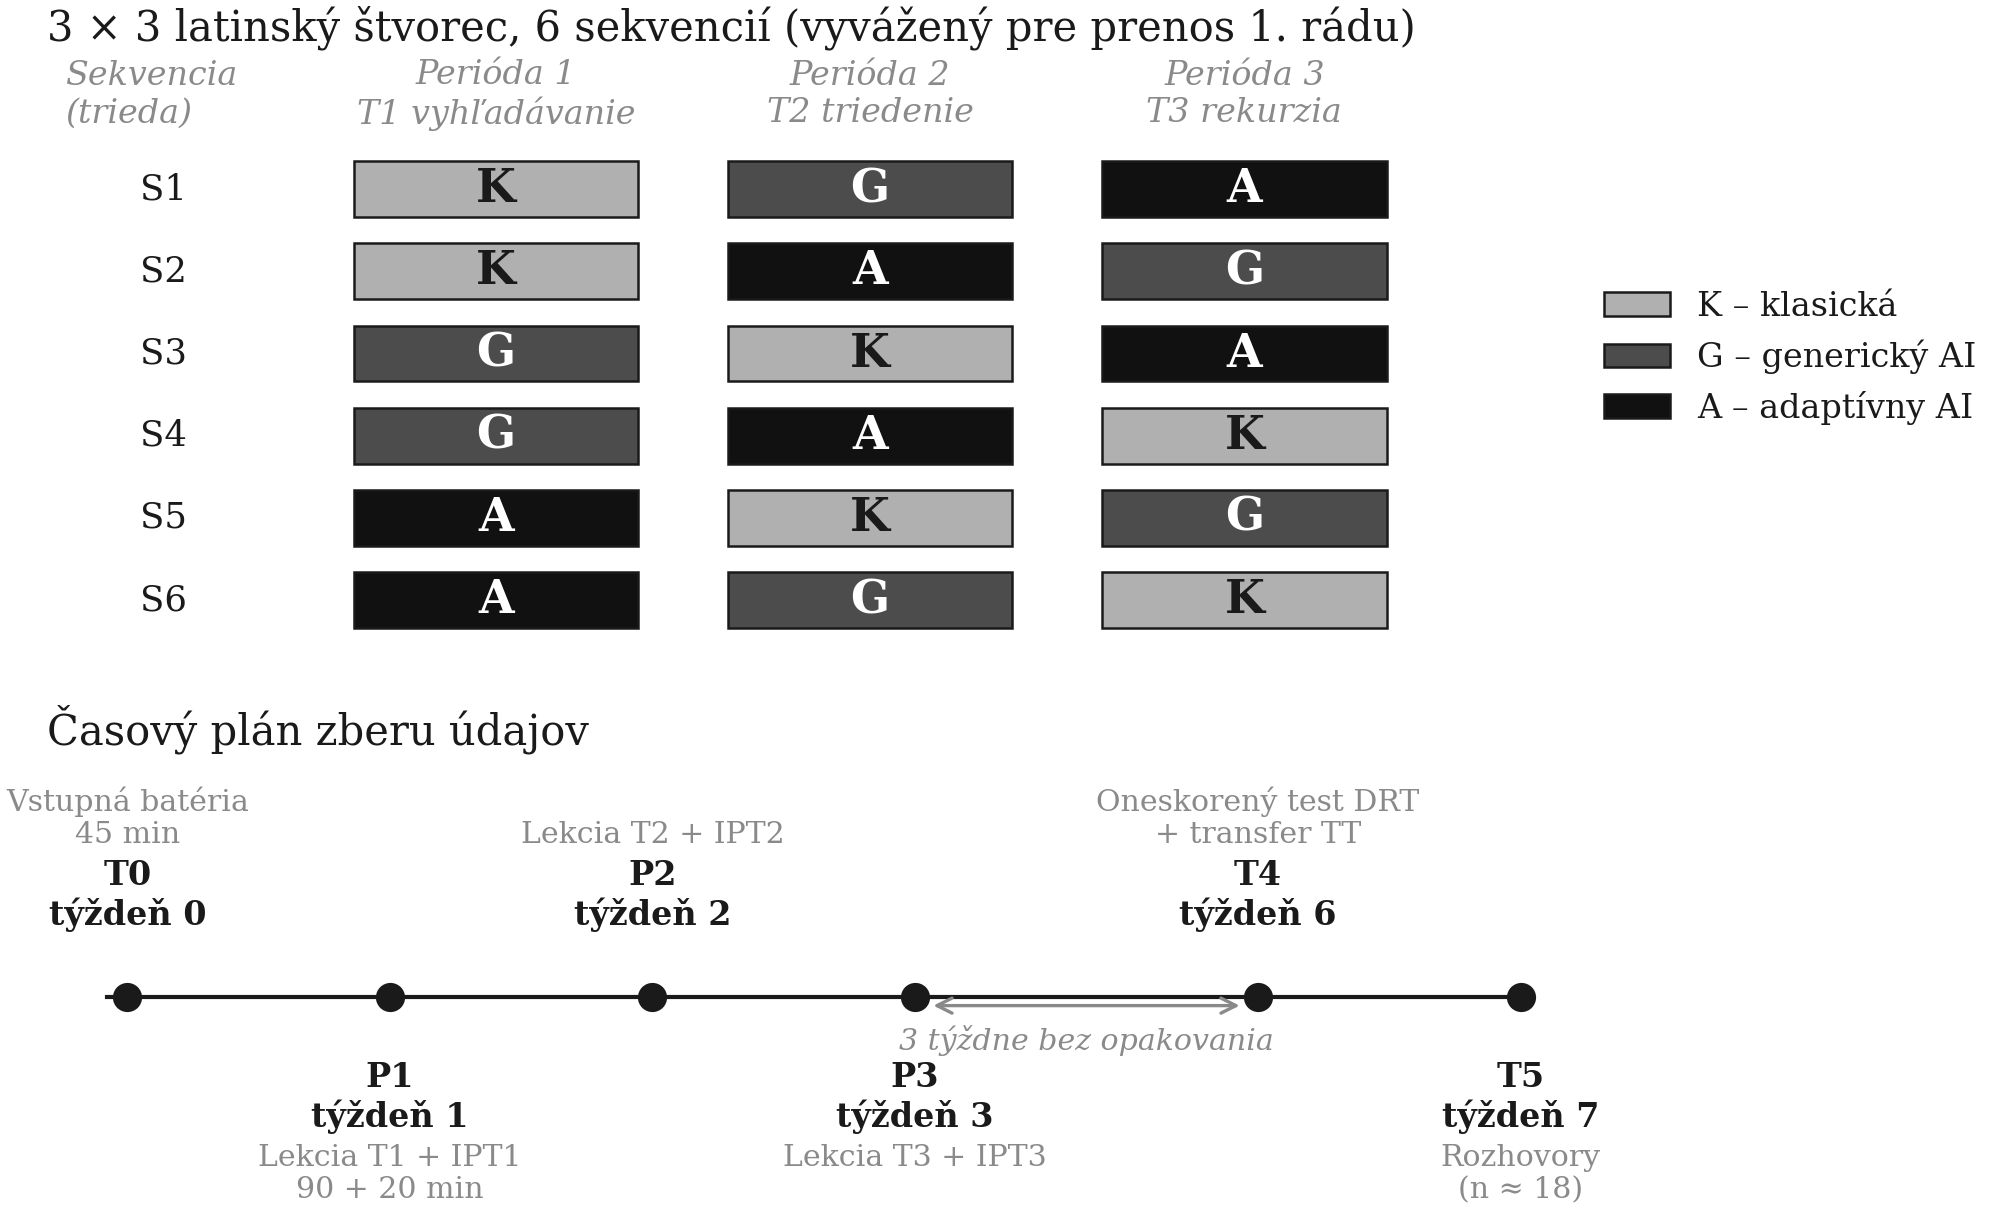
\includegraphics[width=\textwidth]{assets/images/fig_design.png}
    \caption{Usporiadanie experimentu. Hore: latinský štvorec so šiestimi sekvenciami, ktorý vyvažuje podmienku voči perióde aj voči téme a súčasne umožňuje odhadnúť prenos prvého rádu. Dole: časový plán zberu údajov.}
    \label{fig:dizajn}
\end{figure}

\subsection{Prečo krížový dizajn a nie paralelné skupiny}

Voľba krížového dizajnu je v školskom prostredí zásadná z troch dôvodov, z ktorých prvé dva sú metodologické a tretí etický.

\paragraph{Každý žiak je sám sebe kontrolou.} V paralelnom usporiadaní sa účinok podmienky odhaduje z rozdielu medzi žiakmi, a teda je zaťažený celou medziindividuálnou variabilitou vstupných vedomostí, motivácie a fluidného uvažovania. V krížovom dizajne sa odhaduje z vnútroindividuálneho rozdielu, čím sa táto variabilita algebricky eliminuje~\cite{senn2002crossover}. Pri empiricky doloženej korelácii opakovaných meraní okolo $r=0{,}55$ to znamená zhruba dvojnásobnú efektívnu veľkosť vzorky.

\paragraph{Zhluková štruktúra prestáva byť prekážkou.} Prideľovanie na úrovni tried je v školskom výskume nevyhnutnosť~--- triedu nemožno rozdeliť uprostred hodiny. V paralelnom zhlukovo randomizovanom pokuse to znamená návrhový efekt $1+(m-1)\rho$, ktorý pri $m=22$ žiakoch v triede a vnútrotriednej korelácii $\rho=0{,}12$ dosahuje hodnotu $3{,}5$~--- vzorka teda „stratí“ takmer tri štvrtiny svojej informačnej hodnoty~\cite{hedges2007icc,raudenbush1997cluster}. V krížovom dizajne sa triedny intercept vo vnútroindividuálnom rozdiele vykráti a návrhový efekt sa na hlavný kontrast \emph{neuplatní}. Obmedzením zostáva len heterogenita účinku medzi triedami, ktorú modelujeme explicitne a kvantifikujeme v časti~\ref{sec:sila}.

\paragraph{Etický rozmer.} V paralelnom usporiadaní by jedna tretina žiakov absolvovala celý cyklus bez prístupu k nástroju, ktorý sa môže ukázať ako prínosný, a iná tretina bez klasickej výučby. Krížový dizajn zabezpečuje, že \emph{každý} žiak absolvuje všetky tri formy výučby a odnesie si celý obsah učiva. Toto je podmienka, ktorú v pilotnom rozhovore označili oslovení riaditelia škôl za rozhodujúcu pre udelenie súhlasu.

\subsection{Prečo šesť sekvencií}

Krížové dizajny majú jednu známu slabinu: účinok podmienky v neskoršej perióde môže byť ovplyvnený podmienkou z predchádzajúcej periódy (prenos, \emph{carry-over}). Pri troch podmienkach neexistuje trojriadkový latinský štvorec vyvážený pre prenos prvého rádu; vyváženie si vyžaduje všetkých šesť permutácií~\cite{williams1949designs}. Preto priraďujeme triedy k šiestim sekvenciám, čím dosiahneme, že každá podmienka nasleduje po každej inej rovnako často. Prenos je potom odhadnuteľný ako samostatný parameter modelu a jeho neprítomnosť je testovateľná, nie predpokladaná.

Doplnkovo prenos obmedzujeme aj vecne: medzi periódami je týždňový odstup, témy sa obsahovo neprekrývajú a žiaci v podmienke $K$ majú notebooky s rovnakým cvičným rozhraním, len s deaktivovaným panelom asistenta. Posledné opatrenie drží technické prostredie konštantné naprieč podmienkami, takže manipulovaná je výhradne dostupnosť a charakter pomoci, nie prítomnosť techniky.

\subsection{Aliasovanie témy a periódy}

Téma je zámerne viazaná na periódu: všetky triedy preberajú v prvom týždni vyhľadávanie, v druhom triedenie a v treťom rekurziu. Dôvodom je kurikulárna nadväznosť~--- poradie tém nemožno ľubovoľne meniť bez zásahu do tematického plánu školy. Dôsledkom je, že hlavný efekt témy a hlavný efekt periódy sú vzájomne aliasované a nemožno ich oddeliť. Táto strata je akceptovateľná, pretože ani jeden z nich nie je predmetom výskumných otázok. Rozhodujúce je, že \emph{podmienka} je voči perióde ortogonálna, a teda účinok podmienky je odhadnuteľný nezaťažene. Interakciu podmienky s periódou (teda aj s témou) v modeli testujeme a vykazujeme.

\section{Účastníci}
\label{sec:ucastnici}

\paragraph{Cieľová populácia.} Žiaci 2.~a 3.~ročníka slovenských gymnázií a technicky zameraných stredných odborných škôl, ktorí v danom školskom roku absolvujú predmet informatika. Voľba tohto ročníka je motivovaná tým, že učivo algoritmizácie je preň v Štátnom vzdelávacom programe štandardné, žiaci už majú základnú programátorskú skúsenosť, a zároveň ešte nie sú v maturitnom ročníku, kde by dodatočné testovanie predstavovalo neprimeranú záťaž.

\paragraph{Výber vzorky a stratifikácia.} Ide o zámerný (nie pravdepodobnostný) výber škôl, čo je pri školskom experimente prakticky nevyhnutné a treba to otvorene priznať ako obmedzenie zovšeobecniteľnosti. Výber stratifikujeme podľa dvoch znakov, ktoré sú v slovenskom kontexte najsilnejšími prediktormi variability výsledkov: \emph{typ školy} (gymnázium verzus technická SOŠ) a \emph{lokalita} (Bratislavský kraj verzus ostatné kraje). Cieľom je zaradiť aspoň jednu školu z každej kombinácie, aby bolo možné vykazovať, či sa účinok medzi typmi škôl líši.

\paragraph{Prideľovanie.} Prideľovanou jednotkou je trieda, prideľovanou hodnotou je \emph{sekvencia} (nie podmienka). Prideľovanie je blokované podľa školy: v rámci každej školy sa triedy náhodne priradia k rôznym sekvenciám, aby sa školský efekt nezamieňal so sekvenčným. Randomizáciu vykoná skript s uloženým semenom generátora, jeho výstup sa archivuje spolu s dátami.

\paragraph{Veľkosť vzorky.} Cieľom je \textbf{18~tried} (približne 396~zapísaných žiakov, po očakávanom 12\,\% úbytku približne 348 žiakov s kompletnými dátami) z troch až štyroch škôl. Minimálna akceptovateľná veľkosť je 12~tried; zdôvodnenie oboch hodnôt je v časti~\ref{sec:sila}. Keďže viazaným obmedzením nie je počet žiakov, ale počet tried, je pre silu testu výhodnejšie získať viac menších tried než menej veľkých~--- čo je odporúčanie, ktoré ide proti intuícii a bolo odvodené zo simulácie.

\paragraph{Vyraďovacie kritériá.} Zo vzorky vyraďujeme žiakov, ktorí sa nezúčastnili aspoň dvoch z troch vyučovacích blokov (nemajú vnútroindividuálny kontrast), a žiakov, ktorých opatrovník odvolal súhlas. Neúčasť na odloženom teste nie je vyraďovacím kritériom; s takými prípadmi sa zaobchádza podľa časti~\ref{subsec:chybajuce}.

\subsection{Umiestnenie vzorky na národnej škále}
\label{sec:narodne-ukotvenie}

Medzi obmedzeniami práce je uvedené, že školy nie sú vybrané náhodne, pretože náhodný výber škôl v slovenskom školskom výskume nie je uskutočniteľný. Stratifikácia riziko zmierňuje a neodstraňuje ho. Toto obmedzenie sa obvykle vysloví a tým sa s ním skončí~--- čo je bežný osud vety „vzorka nie je reprezentatívna“.

Nechať to tak však nie je nutné. Náhodný výber je nemožný; \emph{zmerať, kde vzorka leží}, nie~--- za predpokladu, že existuje nástroj so zverejnenými položkovými štatistikami z veľkej národnej administrácie. Pre slovenskú informatiku taký nástroj existuje práve jeden: iBobor, ktorého úspešnosti jednotlivých úloh pochádzajú z kohorty rádovo \nanCohort{} žiakov ročne.

\paragraph{Postup.} Do vstupnej hodiny sa zaradí podmnožina úloh iBoboru, ktorých národná úspešnosť je zverejnená. Vzorka sa kalibruje s obtiažnosťami týchto úloh \emph{fixovanými} na národných hodnotách namiesto lokálneho odhadu. Osobné miery žiakov tým padnú na národnú metriku a priemer vzorky sa stáva priamo interpretovateľným: táto vzorka leží na takom a takom percentile národného rozdelenia účastníkov.

\paragraph{Koľko úloh to stojí.} Menej, než by sa čakalo. Smerodajná chyba odhadu polohy klesne pod $0{,}10$ logitu už pri \nanItemsNeeded{} kotviacich úlohách a pri ôsmich je $\nanSe$. Presnosť je teda lacná. Zostáva malé systematické skreslenie $\nanBias$ logitu~--- približne \nanBiasPct{} percentilového bodu~--- ktoré pochádza z odvodenia obtiažnosti z okrajovej úspešnosti a ktoré \emph{pridávaním úloh nezmizne}. Uvádzame ho spolu s odhadom.

\paragraph{Čo je skutočným rizikom.} Nie je ním presnosť, ale posun kohorty. Zverejnené obtiažnosti pochádzajú z iného ročníka. Ak sa jednotlivé úlohy posunú \emph{nezávisle}, posuny sa v priemere cez úlohy do značnej miery vyrušia. Ak sa posunie \emph{celá} kohorta~--- ročník bol celkovo lepší alebo horší~--- posun prejde priamo do odhadu polohy a z ukotvených dát ho nemožno odhaliť. Simulácia ukazuje, že systematický posun zväčšuje rozptyl odhadu naprieč štúdiami \nanDriftRatio-násobne oproti nezávislému. Vykazovaný percentil preto nesie citlivostné pásmo tejto veľkosti a formuluje sa ako rozpätie, nie ako bod.

\paragraph{Čo to nedokáže, povedané priamo.} Referenčnou populáciou sú \emph{účastníci} iBoboru, nie všetci slovenskí žiaci. Účasť je na rozhodnutí školy a žiaka, takže je nadreprezentovaná tými, ktorých učiteľ prihlási. „Národná škála“ tu znamená túto účastnícku populáciu a každá veta práce o percentile to musí uviesť. Číslo má napriek tomu cenu: známa referenčná populácia je viac než neznáma. Postup nerobí vzorku reprezentatívnou~--- to nedokáže nič, čo je k dispozícii~--- ale mení nepreukázateľný predpoklad na vykázané číslo, pri ktorom čitateľ vidí smer a veľkosť odchýlky namiesto toho, aby dúfal, že žiadna nie je.


\section{Učivo, témy a ich výber}
\label{sec:temy}

% TODO (návrh zo 16. 10. 2026, na integráciu):
%   Dizajn sa mení na TRI PREDMETY s jednou témou v každom --
%   informatika (vyhľadávanie v poli), matematika (zložené úrokovanie a
%   exponenciálny rast), fyzika (jednosmerný prúd, sériové a paralelné zapojenie).
%   Text návrhu: drafts/temy-troch-predmetov.md
%   Prepísať túto časť aj časť sec:fyzika (FCI sa nahrádza).

Predmetom výučby je \textbf{algoritmizácia a analýza zložitosti} v rámci predmetu informatika. Voľba domény bola vedená štyrmi kritériami: téma musí byť súčasťou štandardného kurikula; musí byť merateľná objektívnym testom s jednoznačným kľúčom; musí byť dostatočne náročná, aby nevznikol stropový efekt; a musí byť taká, kde generatívny nástroj \emph{skutočne dokáže} poskytnúť hotové riešenie~--- inak by sa manipulácia neuskutočnila.

Tri témy boli vybrané tak, aby mali \emph{izomorfnú štruktúru}. Každá z nich má tvar „naivný postup verzus efektívny postup, prečo je efektívny rýchlejší, a kedy sa ktorý oplatí“:

\begin{description}[leftmargin=1.6cm, style=nextline, nosep]
    \item[T1] \textbf{Vyhľadávanie:} lineárne $\mathcal{O}(n)$ verzus binárne $\mathcal{O}(\log n)$; podmienka usporiadanosti poľa.
    \item[T2] \textbf{Triedenie:} insertion sort $\mathcal{O}(n^2)$ verzus merge sort $\mathcal{O}(n\log n)$; princíp rozdeľuj a panuj.
    \item[T3] \textbf{Rekurzia a memoizácia:} naivné Fibonacciho čísla $\mathcal{O}(2^n)$ verzus memoizované $\mathcal{O}(n)$; prekrývajúce sa podproblémy.
\end{description}

Izomorfia štruktúry je metodologicky podstatná: umožňuje zostaviť \emph{paralelné testové formy} s rovnakou špecifikačnou tabuľkou (tabuľka~\ref{tab:blueprint-gen}), v ktorých si položky zodpovedajú bunka po bunke a líšia sa len obsahom. Bez tejto vlastnosti by rozdiel medzi periódami nebolo možné odlíšiť od rozdielu v obtiažnosti tém.

Riziko, ktoré z voľby vyplýva, je obmedzená zovšeobecniteľnosť mimo algoritmického učiva. Tri témy z jednej domény nedovoľujú tvrdiť nič o dejepise alebo o cudzom jazyku. Toto obmedzenie je vedomé a je cenou za internú validitu; v kapitole~\ref{chapter:conclusion} k nemu formulujeme nadväzujúci výskumný krok.

\paragraph{Zvážená a odložená alternatíva: herný merací nástroj.} Pri konzultácii bola zvažovaná aj možnosť merať kritické myslenie voči výstupom umelej inteligencie herným nástrojom s uzavretými možnosťami~--- žiak rieši prípady s asistentom, ktorý občas klame, a pri každom kroku volí medzi \emph{uveriť}, \emph{overiť}, \emph{spýtať sa} a \emph{odmietnuť}, čo dáva automatické skóre po dimenziách. Prototyp takého nástroja bol vypracovaný. Do tohto dizajnu nebol zaradený z dvoch dôvodov. Po prvé, herné skóre meria \emph{správanie v hre}, ktorého vzťah ku školskému učeniu by bolo treba najprv samostatne validovať~--- pridal by teda neoverený merací nástroj do experimentu, ktorý už jeden neoverený nástroj obsahuje (index PEQI). Po druhé, hra by zabrala vyučovací čas, ktorý potrebuje odložený test. Nástroj však zostáva relevantný ako \emph{nezávislé kritérium} pre validáciu indexu PEQI v nadväzujúcom výskume: ak PEQI skutočne meria to, čo tvrdí, mal by s herným skóre korelovať.

\subsection{Druhý predmet: fyzika a Force Concept Inventory}
\label{sec:fyzika}

Štúdia postavená na jedinom predmete nedovoľuje tvrdiť nič o inom. Obmedzenie je v prácach tohto typu obvyklé a obvykle sa ponechá tak. Tu sa zmierňuje pridaním druhého predmetu~--- fyziky~--- a voľba fyziky má jediný, ale rozhodujúci dôvod: pre ňu existuje validovaný nástroj, ktorý netreba zostavovať.

\paragraph{Force Concept Inventory.} FCI~\cite{hestenes1992fci} je 30\-položkový koncepčný inventár newtonovskej mechaniky, používaný od roku 1992, s normami z desaťtisícov žiakov a s rozsiahlou literatúrou o jeho vlastnostiach. Rozptyľovače nie sú náhodné: každý zodpovedá konkrétnej doloženej miskoncepcii, takže nesprávna odpoveď nesie informáciu o tom, \emph{ako} žiak uvažuje. To je presne vlastnosť, ktorú vlastný test po pol roku vývoja nedosiahne.

\paragraph{Slovenská verzia existuje.} Na portáli PhysPort je dostupný slovenský preklad FCI od J.~Hanča a J.~Tótha~\cite{physport2025fci}. Preklad teda netreba vyrábať. Treba však uviesť dve výhrady, lebo obe menia to, čo z neho možno tvrdiť:

\begin{description}[leftmargin=0.6cm, nosep]
    \item[\textbf{Preklad nie je validácia.}] PhysPort pri prekladoch výslovne uvádza, že neručí za ich presnosť ani platnosť, a že nástroj validovaný pre jeden jazyk a kultúru nemusí byť platný pre iný. Slovenská verzia sa preto v pilote overuje ako ktorýkoľvek iný nástroj: obtiažnosť položiek, zhoda s modelom, a najmä \emph{funkčná odlišnosť položiek} oproti zverejneným medzinárodným hodnotám. Položka, ktorá sa v slovenskom znení správa inak než inde, je podozrivá z chyby prekladu.
    \item[\textbf{Nástroj je chránený.}] FCI sa zámerne nešíri verejne, aby sa položky nedostali k žiakom vopred; prístup je viazaný na overený učiteľský alebo výskumný účet. Z toho plynie, že na rozdiel od ostatných nástrojov tejto práce ho \emph{nemožno} zverejniť spolu s dátami. Táto asymetria sa vykazuje: časť nástrojov práce je plne otvorená, časť nie, a dôvod je v oboch prípadoch uvedený.
\end{description}

\paragraph{Ako sa fyzika vkladá do dizajnu.} Nie ako štvrtá téma do existujúceho štvorca~--- to by rozbilo izomorfiu troch informatických tém, na ktorej stojí vnútroindividuálny kontrast. Fyzika tvorí \emph{paralelné rameno} s vlastným krížovým štvorcom v triedach, ktoré majú fyziku v rovnakom ročníku. Analyzuje sa rovnakým modelom a pridáva jediný nový člen: interakciu \emph{predmet $\times$ podmienka}.

Práve ten člen je dôvodom celého rozšírenia. Ak je účinok pedagogického ohraničenia v informatike a vo fyzike porovnateľný, tvrdenie práce sa netýka algoritmizácie, ale spôsobu práce s nástrojom. Ak sa líši, je to zistenie o doméne a je zaujímavejšie než jednodoménový výsledok.

\paragraph{Čo to stojí a kde je riziko.} Fyzika má na stredných odborných školách podstatne menšiu hodinovú dotáciu než na gymnáziách, takže rameno bude pravdepodobne tvorené prevažne gymnáziami. Vzorka druhého ramena teda nebude mať to isté zloženie ako prvého a porovnanie predmetov je o tento rozdiel zaťažené. Uvádzame to ako obmedzenie dopredu, nie ako zistenie dodatočne: interakcia \emph{predmet $\times$ podmienka} je čiastočne zamenená s typom školy a bez stratifikovaného náboru ju od seba oddeliť nemožno.


\section{Experimentálne podmienky}
\label{sec:podmienky}

Všetky tri podmienky trvajú 90~minút (dve vyučovacie hodiny), prebiehajú v tej istej učebni, s tým istým učiteľom, podľa scenára s rovnakou štruktúrou (35~min výklad~--- 40~min samostatná práca na rovnakej sade úloh~--- 15~min spoločné zhrnutie) a s rovnakými riešenými príkladmi vo výkladovej časti. Podmienky sa líšia \emph{výhradne tým, aká pomoc je dostupná počas 40-minútovej samostatnej práce}. Úplné scenáre sú v prílohe~\ref{chapter:lekcie}.

\subsection{Podmienka K --- klasická výučba}

Žiaci pracujú na tlačenom pracovnom liste a na notebooku s cvičným rozhraním, v ktorom je panel asistenta skrytý. Učiteľ prechádza triedou a odpovedá na otázky tak, ako to robí bežne. Ide teda o \emph{dobre vedenú konvenčnú hodinu}, nie o slamenú figurínu: obsahuje riešené príklady, spätnú väzbu učiteľa aj priestor na otázky. To je zámer~--- ak by kontrolná podmienka bola umelo ochudobnená, akýkoľvek rozdiel v prospech nástroja by bol artefaktom.

\subsection{Podmienka G --- generický nástroj}

Žiaci majú v cvičnom rozhraní otvorený panel s konverzačným asistentom bez akýchkoľvek pedagogických obmedzení: bez systémového promptu obmedzujúceho odpovede, bez nápovedí po krokoch, bez akejkoľvek znalosti o žiakovi. Inštrukcia znie: \emph{„Asistenta môžeš používať tak, ako uznáš za vhodné.“} Učiteľ odpovedá len na organizačné otázky. Táto podmienka zámerne modeluje realitu, ktorá v školách nastáva, keď si žiak otvorí verejne dostupný konverzačný systém.

\subsection{Podmienka A --- adaptívny (sokratovský) nástroj}

Žiaci pracujú v tom istom rozhraní, s tým istým základným modelom a na tej istej sade úloh. Pedagogická vrstva medzi žiakom a modelom pridáva tri mechanizmy:

\begin{enumerate}[nosep]
    \item \textbf{Systémový prompt so zákazom hotového riešenia.} Asistent nesmie vydať úplné riešenie ani finálnu číselnú odpoveď. Na každý dopyt najprv odpovedá diagnostickou otázkou a následne nápoveďami so stupňovanou konkrétnosťou (od pripomenutia princípu cez zúženie miesta chyby až po ukážku analogického, nie totožného, prípadu). Úplné znenie promptu je v prílohe~\ref{sec:sysprompt}.
    \item \textbf{Vrstva modelu znalostí žiaka.} Jednoduchý model sledovania znalostí (Bayesian knowledge tracing) odhaduje pravdepodobnosť zvládnutia každej z piatich čiastkových zručností a na jej základe vyberá ďalšiu úlohu aj úroveň, na ktorej začína nápoveda. Tým sa realizuje adaptivita v presnom zmysle~--- prispôsobenie \emph{postupnosti}, nie len formulácie.
    \item \textbf{Brána vlastného vysvetlenia.} Pred odomknutím vzorového riešenia musí žiak napísať aspoň jednu vetu, v ktorej vlastnými slovami uvedie, prečo je jeho postup správny alebo kde predpokladá chybu. Ide o priamu implementáciu efektu vlastného vysvetľovania~\cite{fiorella2016generative,chi2014icap}.
\end{enumerate}

\paragraph{Prečo je toto porovnanie čistejšie než v doterajšej literatúre.} Štúdia Slijepcevica a Yaylaliho~\cite{slijepcevic2025khanmigo} porovnávala Khanmigo s Googlom, čím naraz menila model, rozhranie, obsah aj pedagogiku~--- prípadný rozdiel nemožno pripísať žiadnemu z nich. V našom usporiadaní sú model, rozhranie, úlohy, učiteľ aj čas identické a mení sa \emph{výlučne pedagogická vrstva}. Ak sa podmienky $G$ a $A$ budú líšiť, je to dôkaz o účinku pedagogického ohraničenia, nie o kvalite modelu. Táto vlastnosť je hlavným metodologickým prínosom dizajnu.

\paragraph{Vernosť realizácie.} Každú hodinu pozoruje nezávislý pozorovateľ a vypĺňa dvanásťpoložkový protokol vernosti (príloha~\ref{sec:vernost}): dodržanie časovania jednotlivých blokov, dodržanie scenára výkladu, neposkytnutie riešenia učiteľom, funkčnosť panela asistenta a podobne. Vykazujeme podiel dodržaných položiek a v citlivostnej analýze opakujeme hlavný model len na hodinách s vernosťou nad 90\,\%.

\section{Meranie}
\label{sec:meranie}

Prehľad všetkých meraných veličín je v tabuľke~\ref{tab:premenne}. Plné znenie položiek je v prílohe~\ref{chapter:instrumenty}.

\begin{table}[H]
\centering
\caption{Prehľad meraných premenných}
\label{tab:premenne}
\small
\begin{tabularx}{\textwidth}{@{}l l X l@{}}
\toprule
\textbf{Skratka} & \textbf{Kedy} & \textbf{Čo meria} & \textbf{Rozsah} \\
\midrule
\multicolumn{4}{@{}l}{\textit{Učebné výsledky}} \\
PRAC   & počas hodiny & úspešnosť riešenia cvičných úloh & 0--1 \\
IPT    & +0 min       & okamžitý test, \asmFormItems{} položiek, Raschova škála & $\theta$ \\
DRT    & +3 týždne    & odložené vybavenie, \asmFormItems{} položiek na tému & $\theta$ \\
TT     & +3 týždne    & vzdialený transfer, \instrTtItems{} položiek & $\theta$ \\
\midrule
\multicolumn{4}{@{}l}{\textit{Metakognícia}} \\
JOL    & pri položke  & sebadôvera v správnosť odpovede & 0--100 \\
BIAS   & odvodené     & JOL $-$ skutočná úspešnosť (nadhodnotenie) & $[-1,1]$ \\
ABS    & odvodené     & priemerná absolútna kalibračná chyba & $[0,1]$ \\
GAMMA  & odvodené     & rozlišovacia schopnosť (Goodman--Kruskal $\gamma$) & $[-1,1]$ \\
FOL    & po hodine    & subjektívny pocit naučenia & 1--7 \\
\midrule
\multicolumn{4}{@{}l}{\textit{Proces (len $G$ a $A$)}} \\
PEQI   & z logov      & epistemická kvalita promptov & 0--1 \\
OR     & z logov      & podiel offloadingových promptov & 0--1 \\
$T_1$  & z logov      & čas do prvého promptu po zadaní úlohy & s \\
VTR    & z logov      & doslovný prenos výstupu do odpovede žiaka & 0--1 \\
ABHR   & z logov      & podiel úloh s vlastným pokusom pred prvým promptom & 0--1 \\
\midrule
\multicolumn{4}{@{}l}{\textit{Záťaž, postoje, kovariáty}} \\
CL$_{\mathrm{i,e,g}}$ & po hodine & vnútorná / vonkajšia / germánna záťaž & 0--10 \\
SAT    & po hodine    & spokojnosť s formátom hodiny & 1--7 \\
$\theta_{\mathrm{pre}}$ & pred každou témou & vstupné vedomosti \emph{k danej téme}, 5 položiek & $\theta$ \\
$g_f$  & T0a a T4     & fluidné uvažovanie, ICAR, \mplGfItems{} položiek & $z$ \\
CT     & T0a (T6)     & informatické myslenie, iBobor, 8 úloh & $\theta$ \\
MAI    & T0b          & metakognitívna uvedomelosť, Jr.~MAI, \instrMaiItems{} položiek & 1--5 \\
\bottomrule
\end{tabularx}
\end{table}

\subsection{Učebné výsledky}

\paragraph{Testové formy a ich zostavenie.} Pre každú tému existujú dve formy, okamžitá (IPT) a odložená (DRT), obe s~\asmFormItems{}~položkami, s~jednou špecifikačnou tabuľkou a s~rovnakým počtom rubrikových položiek (\asmOpenPerForm). Kotviacich položiek je \asmAnchors{} a \emph{v~oboch formách sú znak po znaku totožné}. Sú tým, čo obe formy robí porovnateľnými, a totožnosť nie je tvrdenie v~texte: zásobník položiek odmietne načítať sadu, v~ktorej sa hoci jedna kotviaca položka medzi formami líši.

To treba povedať takto dôrazne preto, že predchádzajúca verzia tejto práce totožnosť tvrdila na dvoch miestach a nemala ju ani raz~--- okamžitá forma sa pýtala na pole s~1024 prvkami, odložená na pole s~512, a jedna „kotviaca“ položka mala v~jednej forme štyri možnosti a v~druhej voľnú numerickú odpoveď. Pri pol logitu rozdielu by sa znak primárneho kontrastu obrátil: štúdia by vykázala zlepšenie tam, kde v~skutočnosti nastalo zabúdanie. Celé vyčíslenie je v~prílohe~\ref{chapter:hodnotiaci-modul}, časti~\ref{sec:kotvenie-oprava}.

Kotvia sa výhradne uzavreté položky. Pri rubrikovej položke by do prevodu oboch foriem na spoločnú škálu vstúpila aj zhoda medzi hodnotiteľmi, takže chyba merania hodnotenia by sa stala chybou prepojenia škál.

Ide o krok, ktorý sa v školskom výskume bežne vynecháva, a jeho vynechanie je fatálne. Ak sa obe formy kalibrujú samostatne, každá z nich je definitoricky vycentrovaná na vlastnú priemernú obtiažnosť; rozdiel medzi okamžitým a odloženým skóre potom zamieňa zabúdanie s tým, ktorý test bol náhodou ťažší. Keďže celé tvrdenie práce spočíva práve na tomto rozdiele, kotvenie nemožno predpokladať~--- treba ho vykonať. V analýze sa preto obe formy kalibrujú \emph{súbežne} v jednom modeli, v ktorom kotviace položky vystupujú ako tie isté položky na oboch príležitostiach a ostatné ako nezadané. Ide o prepojenie foriem spoločnými položkami v zmysle Kolena a Brennana~\cite{kolen2014equating}. Overenie, že postup skutočne obnoví veľkosť zabudnutia, je v časti~\ref{sec:ekvivalencia-overenie}.

\paragraph{Špecifikačná tabuľka.} Položky sú rozdelené podľa kognitívnej úrovne tak, aby test nemeral len zapamätanie postupu. Rozdelenie je \emph{jedno} pre obe formy a pre všetky tri témy, čo je predpokladom izomorfie foriem; tabuľka je generovaná zo zásobníka položiek a je v~prílohe~\ref{chapter:instrumenty} (tabuľka~\ref{tab:blueprint-gen}). Tu ju neuvádzame zámerne: vytlačiť ju na dvoch miestach znamená mať dve kópie jednej špecifikácie, a to je presne tá chyba, pre ktorú kotvenie foriem v~tejto práci raz neexistovalo (príloha~\ref{chapter:hodnotiaci-modul}, časť~\ref{sec:kotvenie-oprava}).

\paragraph{Transferový test.} Šesť položiek TT používa algoritmy, ktoré sa \emph{nepreberali}~--- interpolačné vyhľadávanie, skokové vyhľadávanie, počítanie v inak štruktúrovanom cykle. Žiak nemôže vybaviť naučený postup; musí preniesť princíp. Toto je meranie, na ktorom by sa podľa hypotézy H4 mal rozdiel medzi generatívnou a offloadingovou interakciou prejaviť najsilnejšie.

\paragraph{Skórovanie.} Uzavreté položky sa skórujú 0/1. Položky na úrovni Hodnotenie sa skórujú podľa rubriky (0--2 body) dvoma nezávislými hodnotiteľmi; vykazuje sa medzihodnotiteľská zhoda. Primárnym ukazovateľom je Raschova osobná miera $\theta$~\cite{boone2016rasch}, ktorá na rozdiel od percentuálnej úspešnosti nepredpokladá, že všetky položky sú rovnako ťažké, a poskytuje intervalovú škálu. Ako sekundárny, ľahšie interpretovateľný ukazovateľ vykazujeme aj hrubú úspešnosť a normalizovaný zisk podľa Hakea~\cite{hake1998interactive}.

\paragraph{Kontrola kvality položiek.} Pred akoukoľvek analýzou účinkov sa pre každú položku počítajú ukazovatele zhody s modelom: \emph{infit} a \emph{outfit} ako vážený a nevážený priemer štvorcov štandardizovaných rezíduí. Outfit je citlivý na náhodné uhádnutia slabých žiakov, infit na nezhodu u žiakov, na ktorých je položka zacielená. Pásmo prijateľnosti $0{,}7$ až $1{,}3$ zodpovedá bežnému odporúčaniu pre testy s uzavretými položkami~\cite{linacre2002fit,wright1979besttest}; položky mimo neho sa z merania vylučujú a ich zoznam sa vykazuje.

\paragraph{Funkčná odlišnosť položiek.} Položka, ktorá sa správa inak podľa toho, ktorú hodinu žiak absolvoval, robí z rozdielu medzi podmienkami čiastočne artefakt nástroja. Pre každú položku preto odhadujeme obtiažnosť osobitne v podmienke $A$ a v podmienke $G$ pri osobných mierach fixovaných na spoločnej škále a vykazujeme posun v obvyklých pásmach ($|{\Delta b}| < 0{,}43$ zanedbateľný, do $0{,}64$ stredný, nad $0{,}64$ veľký)~\cite{zieky2003dif}. Položky s veľkým posunom sa vylučujú.

\subsection{Metakognícia a kalibrácia}
\label{subsec:metakognicia}

Toto je meranie, ktorým operacionalizujeme „ilúziu porozumenia“. Po každej položke okamžitého testu žiak posunie jazdec na otázku \emph{„Nakoľko si si istý/á, že tvoja odpoveď je správna?“} v rozsahu 0--100. Z tejto položkovej sebadôvery a zo skutočnej správnosti počítame tri odlišné a nezameniteľné veličiny~\cite{schraw2009conceptual}:

\begin{description}[leftmargin=2.4cm, style=nextline, nosep]
    \item[Skreslenie] $\mathrm{BIAS}=\overline{\mathrm{JOL}}-\overline{\text{správnosť}}$. Kladná hodnota znamená nadhodnotenie. Toto je ukazovateľ, ktorý priamo zodpovedá hypotéze H5.
    \item[Absolútna presnosť] $\mathrm{ABS}=\overline{\lvert \mathrm{JOL}_i-\text{správnosť}_i\rvert}$. Meria, ako veľmi sa žiak mýli v odhade, bez ohľadu na smer.
    \item[Rozlišovacia schopnosť] Good\-man\--Krus\-ka\-lo\-va $\gamma$ medzi se\-ba\-dô\-ve\-rou a správ\-nos\-ťou \emph{v rámci} žiaka~\cite{nelson1984gamma}. Meria, či žiak aspoň \emph{vie rozlíšiť}, ktorým odpovediam má veriť. Žiak môže byť silne nadhodnotený, a pritom mať dobrú rozlišovaciu schopnosť~--- ide o nezávislé vlastnosti.
\end{description}

Doplnkovo sa zaznamenáva globálny odhad pred testom („Koľko zo 16 otázok zodpovieš správne?“) a po hodine subjektívny pocit naučenia a spokojnosť. Formálnym testom disociácie je interakcia \emph{podmienka $\times$ typ ukazovateľa} na štandardizovaných hodnotách pocitu naučenia a odloženého výkonu (časť~\ref{subsec:kontrasty}).

Teoretickým podkladom je model využitia vodidiel~\cite{koriat1997monitoring}: sebadôvera sa neodvodzuje z obsahu pamäte, ale z plynulosti spracovania. Generatívny nástroj plynulosť maximalizuje, a preto by mal sebadôveru nadhodnocovať silnejšie než ktorákoľvek iná podmienka. Praktický dôsledok je nepríjemný: bežné nástroje hodnotenia kvality hodiny~--- dotazník spokojnosti žiakov~--- budú pri zavádzaní nástrojov umelej inteligencie systematicky uprednostňovať horšiu možnosť~\cite{deslauriers2019feeling,dunlosky2012overconfidence}.

\section{Čo presne meriame, keď hovoríme o kognitívnych schopnostiach}
\label{sec:konstrukty}

Spojenie „zmeny kognitívnych schopností žiakov“ nepomenúva jednu merateľnú veličinu. Pomenúva najmenej štyri, ktoré sa líšia rýchlosťou zmeny o dva rády~--- a práve tento rozdiel rozhoduje o tom, ako sa dajú merať a či sa vôbec dajú. Táto časť ten rozdiel vyslovuje explicitne, pretože bez neho je celý merný plán nekontrolovateľný.

\begin{table}[H]
\centering
\caption{Hierarchia konštruktov, rýchlosť ich zmeny a úloha v dizajne}
\label{tab:konstrukty}
\small
\begin{tabularx}{\textwidth}{@{}l X l l@{}}
\toprule
\textbf{Vrstva} & \textbf{Konštrukt} & \textbf{Horizont zmeny} & \textbf{Úloha} \\
\midrule
L0 & fluidné uvažovanie ($g_f$) & roky & kovariát + negatívna kontrola \\
L1 & informatické a algoritmické myslenie & mesiace & kovariát (+ voliteľný výstup) \\
L2 & vedomosti k preberanej téme & jedna hodina & \textbf{primárny výstup} \\
L3 & stratégia: offloading, kalibrácia & jedna úloha & mechanizmus, H5, H6 \\
\bottomrule
\end{tabularx}
\end{table}

\paragraph{Pravidlo, ktoré z toho plynie.} \emph{Interval merania musí zodpovedať rýchlosti zmeny konštruktu.} Trojtýždňová štúdia nedokáže zmerať zmenu na vrstve L0 a žiadny nástroj to nenapraví, pretože nejde o vlastnosť nástroja, ale o vlastnosť konštruktu. Dizajn, ktorý by tvrdil opak, nie je nedostatočne silný~--- meria niečo iné, než o čom hovorí. Literatúra o tréningu kognitívnych schopností je v tomto bode jednoznačná: blízky prenos sa dosahuje, vzdialený prakticky nie.

Z toho plynie rozdelenie úloh. Na vrstvách L2 a L3 sa \emph{merá zmena}; to sú výstupy tejto práce. Na vrstvách L0 a L1 sa \emph{meria stabilita}~--- slúžia ako kovariáty a $g_f$ navyše ako negatívna kontrola (časť~\ref{sec:negativne-kontroly}). Tvrdenie „nezmenilo sa to“ je však tvrdenie ako každé iné a má vlastnú požiadavku na presnosť, ktorú rozoberáme nižšie.

\subsection{Požiadavka na spoľahlivosť sa líši podľa úlohy, nie podľa zvyklosti}

Hranica „$\alpha \geq 0{,}7$“ nie je požiadavka, je to heslo. Každá z troch úloh vyžaduje niečo iné a každá inú hodnotu:

\begin{description}[leftmargin=0.6cm, nosep]
    \item[\textbf{Výstup}] musí zachytiť \emph{zmenu}. Spoľahlivosť rozdielového skóre je podstatne nižšia než spoľahlivosť jednotlivých meraní, takže pod $0{,}80$ na jednu príležitosť prestáva rozdiel žiakov usporadúvať.
    \item[\textbf{Kovariát}] odstraňuje zmätenie len v podiele rovnom vlastnej spoľahlivosti. Pri $0{,}75$ teda štvrtina zmätenia v dátach zostáva~--- a zostáva v podobe, ktorá vyzerá presne ako účinok.
    \item[\textbf{Negatívna kontrola}] musí byť schopná \emph{prejsť}. Toto je smer, ktorý sa najčastejšie pomýli: nepresná kontrola nespôsobuje falošné poplachy, ale rozšíri interval natoľko, že sa už nezmestí do pásma ekvivalencie. Zlyháva teda tým, že nikdy nič nepotvrdí, čo vo výsledkovej tabuľke vyzerá ako nevysvetlená anomália, nie ako problém merania.
\end{description}

Pôvodný plán predpisoval dvanásť matíc. Pri tejto dĺžke vychádza spoľahlivosť $\mplRelTwelve$, čo nestačí ani na jednu z dvoch úloh, ktoré mal nástroj plniť. Pri dvadsiatich položkách je to $\mplRelGf$ a kontrola prejde v $\mplClearGf$ prípadov, keď je pravda nula. Závislosť je vyčíslená v tabuľke~\ref{tab:spolahlivost}; pod hodnotou $0{,}80$ sa kontrola stáva nepoužiteľnou.

\begin{table}[H]
\centering
\caption{Pravdepodobnosť, že negatívna kontrola prejde, podľa spoľahlivosti nástroja}
\label{tab:spolahlivost}
\small
\begin{tabular}{@{}lcccccc@{}}
\toprule
spoľahlivosť (test--retest) & 0,50 & 0,60 & 0,70 & 0,80 & 0,85 & 0,90 \\
\midrule
kontrola prejde & \mplClearFifty & \mplClearSixty & \mplClearSeventy & \mplClearEighty & \mplClearEightyFive & \mplClearNinety \\
\bottomrule
\end{tabular}
\end{table}

\paragraph{Odhadovaná veličina nie je úroveň, ale zmena.} Črta sa meria \emph{raz} na príležitosť, takže vnútroindividuálny kontrast medzi podmienkami na nej neexistuje~--- pokus o taký kontrast dá veličinu, ktorá je konštrukčne nulová, prejde čímkoľvek a netestuje nič. Odhadnuteľný je kontrast \emph{medzi} žiakmi, kľúčovaný podmienkou poslednej periódy, ktorá sa líši podľa sekvencie, a sekvencia je randomizovaná. Aj tak však platí druhé obmedzenie: na \emph{úrovni} má $g_f$ medziindividuálnu smerodajnú odchýlku okolo jednotky plus triednu zložku, čo sa pri osemnástich triedach do pásma ekvivalencie nezmestí. Analyzuje sa preto \emph{zmena} $T4-T0$, ktorá stabilnú časť vrátane triednej zložky vykráti a ponechá zvyšok $\sqrt{2(1-\rho)}$. Práve toto robí kontrolu použiteľnou~--- a je k dispozícii len preto, že sa črta administruje dvakrát.

\subsection{Nemennosť merania v čase}

Rozdielové skóre má zmysel len vtedy, ak sa parametre položiek medzi príležitosťami nezmenili. Práca doteraz testovala odlišné fungovanie položiek medzi \emph{podmienkami}, nie medzi \emph{príležitosťami}~--- čím nechávala neoverený práve ten kontrast, o ktorý jej ide. Doplňame preto kontrolu posunu obtiažnosti kotviacich položiek, ktoré sú jediné prítomné na oboch príležitostiach, a teda jediné, na ktorých je posun vôbec identifikovateľný.

Kritériom nie je štatistická významnosť, ale pásmo ETS: položka sa označí, ak sa jej obtiažnosť posunie o viac než $0{,}64$ logitu. Dôvod je vecný. Pri $\mplNpupils$ žiakoch je smerodajná chyba posunu jednej položky $\mplDriftSe$ logitu, takže Bonferroniho korigovaný test by zachytil až posun nad $\mplDriftBonf$~--- teda väčší než pásmo, ktoré má strážiť. Testovanie významnosti je tu preto nesprávny nástroj. Pri posune $0{,}8$ logitu sa položka označí s pravdepodobnosťou $\mplDriftPower$ a priemerný počet falošne označených položiek na štúdiu je $\mplDriftFalse$.

\subsection{Voľba nástrojov a ich dostupnosť na Slovensku}

Nástroj, ktorý nemá slovenskú verziu, licenciu alebo administračný čas, nie je nástroj, ale zámer. Tabuľka~\ref{tab:nastroje} uvádza pre každú vrstvu konkrétnu voľbu spolu s tým, čo jej zavedenie v skutočnosti vyžaduje.

\begin{table}[H]
\centering
\caption{Nástroje podľa vrstvy, s licenciou a slovenskou dostupnosťou}
\label{tab:nastroje}
\scriptsize
\begin{tabularx}{\textwidth}{@{}l l c X@{}}
\toprule
\textbf{Vrstva} & \textbf{Nástroj} & \textbf{Položky} & \textbf{Licencia a dostupnosť} \\
\midrule
L0 & ICAR (matice + rady) & \mplGfItems & verejná doména, bez poplatku; položky sú figurálne a číselné, prekladá sa len inštrukcia \\
L1 & iBobor / Bebras & 8 (15 v~semestrálnom ramene) & slovenské zadania, vekové kategórie, viac než 600~úloh v~EduPage; súhlas organizátorov z~FMFI UK \\
L2 & vlastné testy IPT/DRT/TT & 16 / 12 / 6 & vlastné, Raschovsky kalibrované, šesť kotviacich položiek \\
L3 & JOL posuvník & pri položke & vlastný, nesie sa na vedomostnom teste \\
L3 & PEQI zo zachytených promptov & --- & vlastný, pozorovaný; nestojí ani minútu hodiny \\
L3 & Jr.~MAI verzia B & 18 & voľne pre výskum; vyžaduje preklad a spätný preklad \\
\bottomrule
\end{tabularx}
\end{table}

\paragraph{Prečo ICAR a nie Ravenove matice.} Ravenove progresívne matice sú licencované a platené za hárok, čo pri 330~žiakoch a dvoch príležitostiach nie je zanedbateľná položka rozpočtu a navyše bráni zverejneniu nástroja spolu s dátami. ICAR~\cite{condon2014icar} je vo verejnej doméne, bez poplatku a bez obmedzenia na zverejnenie. Položky sú figurálne a číselné, takže nenesú jazykovú záťaž~--- čo je v populácii s časťou žiakov vyučovaných v inom než materinskom jazyku podstatné.

\paragraph{Prečo iBobor.} Ide o rozhodujúcu praktickú výhodu, ktorú nemá žiadny iný nástroj v tomto pláne. Súťaž iBobor prevádzkovaná FMFI~UK zapojila v ročníku 2025 približne 141\,000 žiakov z 1\,634~škôl, prebieha v prostredí EduPage, ktoré väčšina slovenských škôl už používa, a viac než 600~úloh z minulých ročníkov je učiteľom dostupných celoročne. Úlohy sú v slovenčine, členené podľa vekových kategórií, opatrené metaúdajmi o tom, ktoré informatické pojmy obsahujú, a ich úspešnosť je známa z kohorty tej veľkosti. Nijaký nástroj, ktorý by sme zostavili sami, nemôže mať porovnateľnú slovenskú normatívnu základňu.

Súťažné bodovanie iBoboru však \emph{nepreberáme}. Obsahuje zápornú penalizáciu za nesprávnu odpoveď a počiatočný bonus, čo je schéma navrhnutá pre súťaž, nie pre meranie: penalizácia zamieňa vedomosti s ochotou riskovať. Položky preto skórujeme 0/1 a kalibrujeme Raschovým modelom ako ktorýkoľvek iný test.

\paragraph{Priznané napätie pri Jr.~MAI.} Práca stojí na tvrdení, že sebahodnotenie je nesprávny nástroj na meranie kognitívneho offloadingu. Použiť sebahodnotiaci dotazník metakognitívnej uvedomelosti je preto potrebné odôvodniť: pripúšťame ho výhradne ako \emph{črtový kovariát} a nikdy ako výstup. Napätie uvádzame, nie zakrývame.


\section{Tri vrstvy merania a kategorizácia používateľov}
\label{sec:tri-vrstvy}

Zadanie práce žiada od navrhnutého riešenia tri veci: systematický zber údajov, \emph{kategorizáciu používateľov} a meranie zmien vo vybraných schopnostiach pred a po použití nástroja. Táto časť rozoberá druhú a tretiu; prvá je predmetom kapitoly~\ref{chapter:problem}.

Meranie je usporiadané do troch vrstiev. Usporiadanie nie je organizačné~--- každá vrstva odpovedá na inú otázku, mení sa inou rýchlosťou a vyžaduje iný typ nástroja.

\begin{table}[H]
\centering
\caption{Tri vrstvy merania}
\label{tab:vrstvy}
\small
\begin{tabularx}{\textwidth}{@{}l X X l@{}}
\toprule
\textbf{Vrstva} & \textbf{Čo meria} & \textbf{Príklad výskumnej otázky} & \textbf{Typ nástroja} \\
\midrule
\textbf{A}~--- vedomosti (doménové) & koľko sa žiak naučil o konkrétnej téme & „Naučí sa žiak binárne vyhľadávanie lepšie s nástrojom alebo bez neho?“ & doménový test, concept inventory \\
\textbf{B}~--- prenositeľné myslenie & kritické myslenie a metakognícia; ako žiak premýšľa nezávisle od témy & „Oslabuje časté používanie schopnosť posúdiť tvrdenie?“ & scenárový test kritického myslenia, kalibrácia \\
\textbf{C}~--- vzťah k nástroju & nakoľko sa naň žiak spolieha, či mu dôveruje a či mu rozumie & „Existuje skupina žiakov, ktorá slepo dôveruje a zároveň horšie uvažuje?“ & škála spoliehania sa, AI gramotnosť, PEQI \\
\bottomrule
\end{tabularx}
\end{table}

\paragraph{Prečo sa fluidné uvažovanie nemeria ako výsledok.} Fluidné uvažovanie ($g_f$, teda to, čo bežne nazývame inteligenciou) do tohto usporiadania ako \emph{výsledok} nepatrí a práca ho tak nepoužíva. Mení sa v horizonte rokov, nie troch týždňov; literatúra o kognitívnom tréningu dokladá blízky prenos a vzdialený prakticky nie. Trojtýždňová štúdia, ktorá by tvrdila, že zmenila inteligenciu, nemeria to, o čom hovorí. $g_f$ preto vstupuje výhradne ako kovariát a ako negatívna kontrola~--- teda ako tvrdenie, že sa \emph{ne}zmenilo (časť~\ref{sec:konstrukty}).

\subsection{Vrstva B: kritické myslenie merané nástrojom, ktorý existuje}

Pre vrstvu B sa ponúkajú zavedené nástroje~--- Halpernov test kritického myslenia (HCTA), Watson\--Glaserov test, prípadne dotazník metakognitívnej uvedomelosti. Žiadny z prvých dvoch však nie je použiteľný tak, ako je. HCTA je licencovaný, platený a normovaný pre populáciu od 18~rokov; vzorka tejto práce je 14--19 rokov. Watson\--Glaser má rovnaké obmedzenia. Použiť nástroj mimo jeho normatívneho rozsahu a vykazovať z neho skóre by znamenalo vykazovať číslo, ktorého význam nie je známy.

Pre vrstvu~B preto zostavujeme vlastný krátky nástroj a validujeme ho v pilote. Jeho opis, všetkých \ctItems{} položiek a validačný postup sú v prílohe~\ref{chapter:kriticke-myslenie}. Rozhodnutie má cenu~--- vlastný nástroj nemá externé normy~--- a má aj zisk: je v slovenčine, je určený pre vekové rozpätie vzorky, je bezplatný a dá sa zverejniť spolu s prácou, čo pri licencovanom nástroji možné nie je.

\subsection{Vrstva C: vzťah k nástroju}

Vrstva~C je tá, ktorú zadanie pomenúva ako kategorizáciu používateľov, a zbiera sa z troch zdrojov, z ktorých dva sú sebahodnotiace a jeden pozorovaný:

\begin{description}[leftmargin=0.6cm, nosep]
    \item[\textbf{Spoliehanie sa na nástroj}] krátkou škálou typov spoliehania~\cite{hou2025reliance}, ktorá rozlišuje reflektívne, opatrné, bezmyšlienkovité a spolupracujúce používanie.
    \item[\textbf{Gramotnosť v oblasti UI}] dotazníkom AILQ~\cite{ng2024ailiteracy}, validovaným pre stredoškolskú populáciu v afektívnej, behaviorálnej, kognitívnej a etickej zložke.
    \item[\textbf{PEQI a procesné ukazovatele}]~--- pozorované, nie vypovedané (časť~\ref{sec:peqi}).
\end{description}

Zmiešanie dvoch sebahodnotiacich zdrojov s pozorovanými je zámerné. Typológia postavená len na sebahodnotení meria to, čo žiaci o sebe hovoria~--- a práve to je vec, ktorej sa táto práca inde vyhýba. Zároveň sa tým otvára overiteľná otázka: žiak, ktorý sa \emph{hlási} k reflektívnemu používaniu a zároveň posiela prompty úrovne $L_0$, je zaujímavý prípad, nie chyba merania.

\subsection{Kategorizácia používateľov}
\label{sec:kategorizacia}

\paragraph{Prečo priemer nestačí.} Otázka z vrstvy~C nie je otázkou o priemere. Je to otázka, či je populácia \emph{zmesou}~--- či existuje podskupina, pre ktorú je generický nástroj škodlivý, zatiaľ čo priemer triedy vyzerá v poriadku. Priemer dokáže zmes úplne skryť: dva profily pohybujúce sa opačným smerom sa vyrušia a štúdia by vykázala „žiadny účinok“ o populácii, v ktorej bola časť žiakov preukázateľne poškodená.

Na simulovaných dátach je to presne tento prípad (tabuľka~\ref{tab:profily-ucinok}): celkový účinok je $\profOverall$ a od nuly nerozlíšiteľný, kým profil „slepo dôverujúci“ stráca $\profHarm$. Rozpätie naprieč profilmi je $\profSpread$.

\begin{table}[H]
\centering
\caption{Účinok generického nástroja podľa profilu žiaka (simulované dáta)}
\label{tab:profily-ucinok}
\small
\begin{tabular}{@{}lcc@{}}
\toprule
\textbf{Profil} & \textbf{Zmena ($G-K$)} & \textbf{$n$} \\
\midrule
kritický používateľ & \profCritical & \profCriticalN \\
priemerný & \profAverage & \profAverageN \\
vyhýbajúci sa & \profAvoid & \profAvoidN \\
slepo dôverujúci & \textbf{\profHarm} & \profHarmN \\
\midrule
\textbf{celkovo} & \profOverall{} (n.~v.) & \profTotalN \\
\bottomrule
\end{tabular}
\end{table}

\paragraph{Metóda.} Latentná profilová analýza (zmes gaussovských rozdelení) nad šiestimi ukazovateľmi vrstvy~C a vrstvy~B, s počtom profilov zvoleným podľa BIC. Profily sú \emph{vopred pomenované}: ich očakávané stredy sú stanovené pred analýzou a fitované profily sa k nim priraďujú podľa vzdialenosti. Pomenovať zhluky až po tom, ako sa na ne pozrieme, je spôsob, ako sa typológia stane nefalzifikovateľnou.

\paragraph{Voľba kovariančnej štruktúry nie je technický detail.} Toto je miesto, kde analýza tohto typu najčastejšie zlyhá, a zlyhá neviditeľne. Overenie prebehlo oproti \emph{vloženej pravde} aj oproti \emph{vloženej neprítomnosti štruktúry}~--- teda oproti jednotnej populácii s korelovanými ukazovateľmi, v ktorej žiadne profily nie sú.

\begin{table}[H]
\centering
\caption{Štyri kovariančné štruktúry proti vloženej pravde a vloženej nule}
\label{tab:kovariancie}
\small
\begin{tabular}{@{}lccc@{}}
\toprule
\textbf{Štruktúra} & \textbf{Rozdelí jednotnú populáciu} & \textbf{Zhoda s pravdou (ARI)} & \textbf{Použiteľná} \\
\midrule
diagonálna & \covDiagNull & \covDiagAri & nie \\
\textbf{zdieľaná (tied)} & \textbf{\covTiedNull} & \textbf{\covTiedAri} & \textbf{áno} \\
úplná & \covFullNull & \covFullAri & nie \\
sférická & \covSphNull & \covSphAri & nie \\
\bottomrule
\end{tabular}
\end{table}

Výsledok je poučný nad rámec tejto práce. Pri \emph{diagonálnej} štruktúre nemôže jediný komponent zachytiť koreláciu medzi ukazovateľmi~--- žiak, ktorý sa viac spolieha, zároveň menej rozumie a horšie formuluje prompty~--- takže model zachytí koreláciu jediným spôsobom, ktorý má k dispozícii: \emph{pridaním komponentov}. Jednotnú populáciu rozdelil na tri profily v $100\,\%$ simulovaných súborov. Tie profily by vyzerali úplne presvedčivo a boli by výlučne artefaktom modelového predpokladu.

Úplná kovariancia problém odstráni a zavedie opačný: $21$~voľných parametrov na komponent znamená, že BIC odmietne pridať aj komponenty, ktoré v dátach skutočne sú. Zdieľaná kovariancia~--- jedna kovariančná matica spoločná pre všetky profily~--- je jediná, ktorá splní obe kritériá, a je to zároveň to, čo klasická latentná profilová analýza robí. Žiadne z týchto dvoch zlyhaní by nebolo viditeľné z jedného fitu na skutočných dátach.

\paragraph{Štatút zistenia.} Pri plánovanej veľkosti vzorky dosahuje typológia zhodu s vloženou pravdou $\profAri$ (upravený Randov index), čo je stredná, nie silná zhoda. Typológia sa preto vykazuje \emph{exploratívne} a nevstupuje do konfirmačnej rodiny. Konfirmačnou by sa stala približne pri \profNeeded{}~žiakoch. To nie je dôvod ju vynechať: výsledok vyššie ukazuje, že priemer triedy je blízky nule, zatiaľ čo jeden profil je zreteľne poškodený~--- dizajn, ktorý by vykazoval len priemery, by túto populáciu opísal nesprávne.


\section{PEQI: index epistemickej kvality promptov}
\label{sec:peqi}

PEQI je hlavným metodologickým prínosom práce. Jeho účelom je nahradiť sebahodnotiace meranie kognitívneho offloadingu~\cite{gerlich2025offloading} meraním \emph{pozorovaným}, ktoré sa počíta automaticky z promptov, ktoré žiak skutočne odoslal.

\subsection{Taxonómia}

Každý prompt sa zaradí do jednej zo šiestich kategórií. Usporiadanie kategórií nie je ľubovoľné~--- opiera sa o rámec ICAP~\cite{chi2014icap}, ktorý radí kognitívne zapojenie od pasívneho cez aktívne a konštruktívne k interaktívnemu. Časť~\ref{sec:icap-rung} rozoberá, ktorú časť tohto usporiadania index skutočne potrebuje a ktorú nie, pretože najvyšší stupienok rámca je sporný a práca sa oň neopiera. Taxonómia je znázornená na obrázku~\ref{fig:peqi}~(a); úplný kódovací manuál s rozhodovacími pravidlami a hraničnými prípadmi je v prílohe~\ref{chapter:kodovaci-manual}.

\begin{figure}[H]
    \centering
    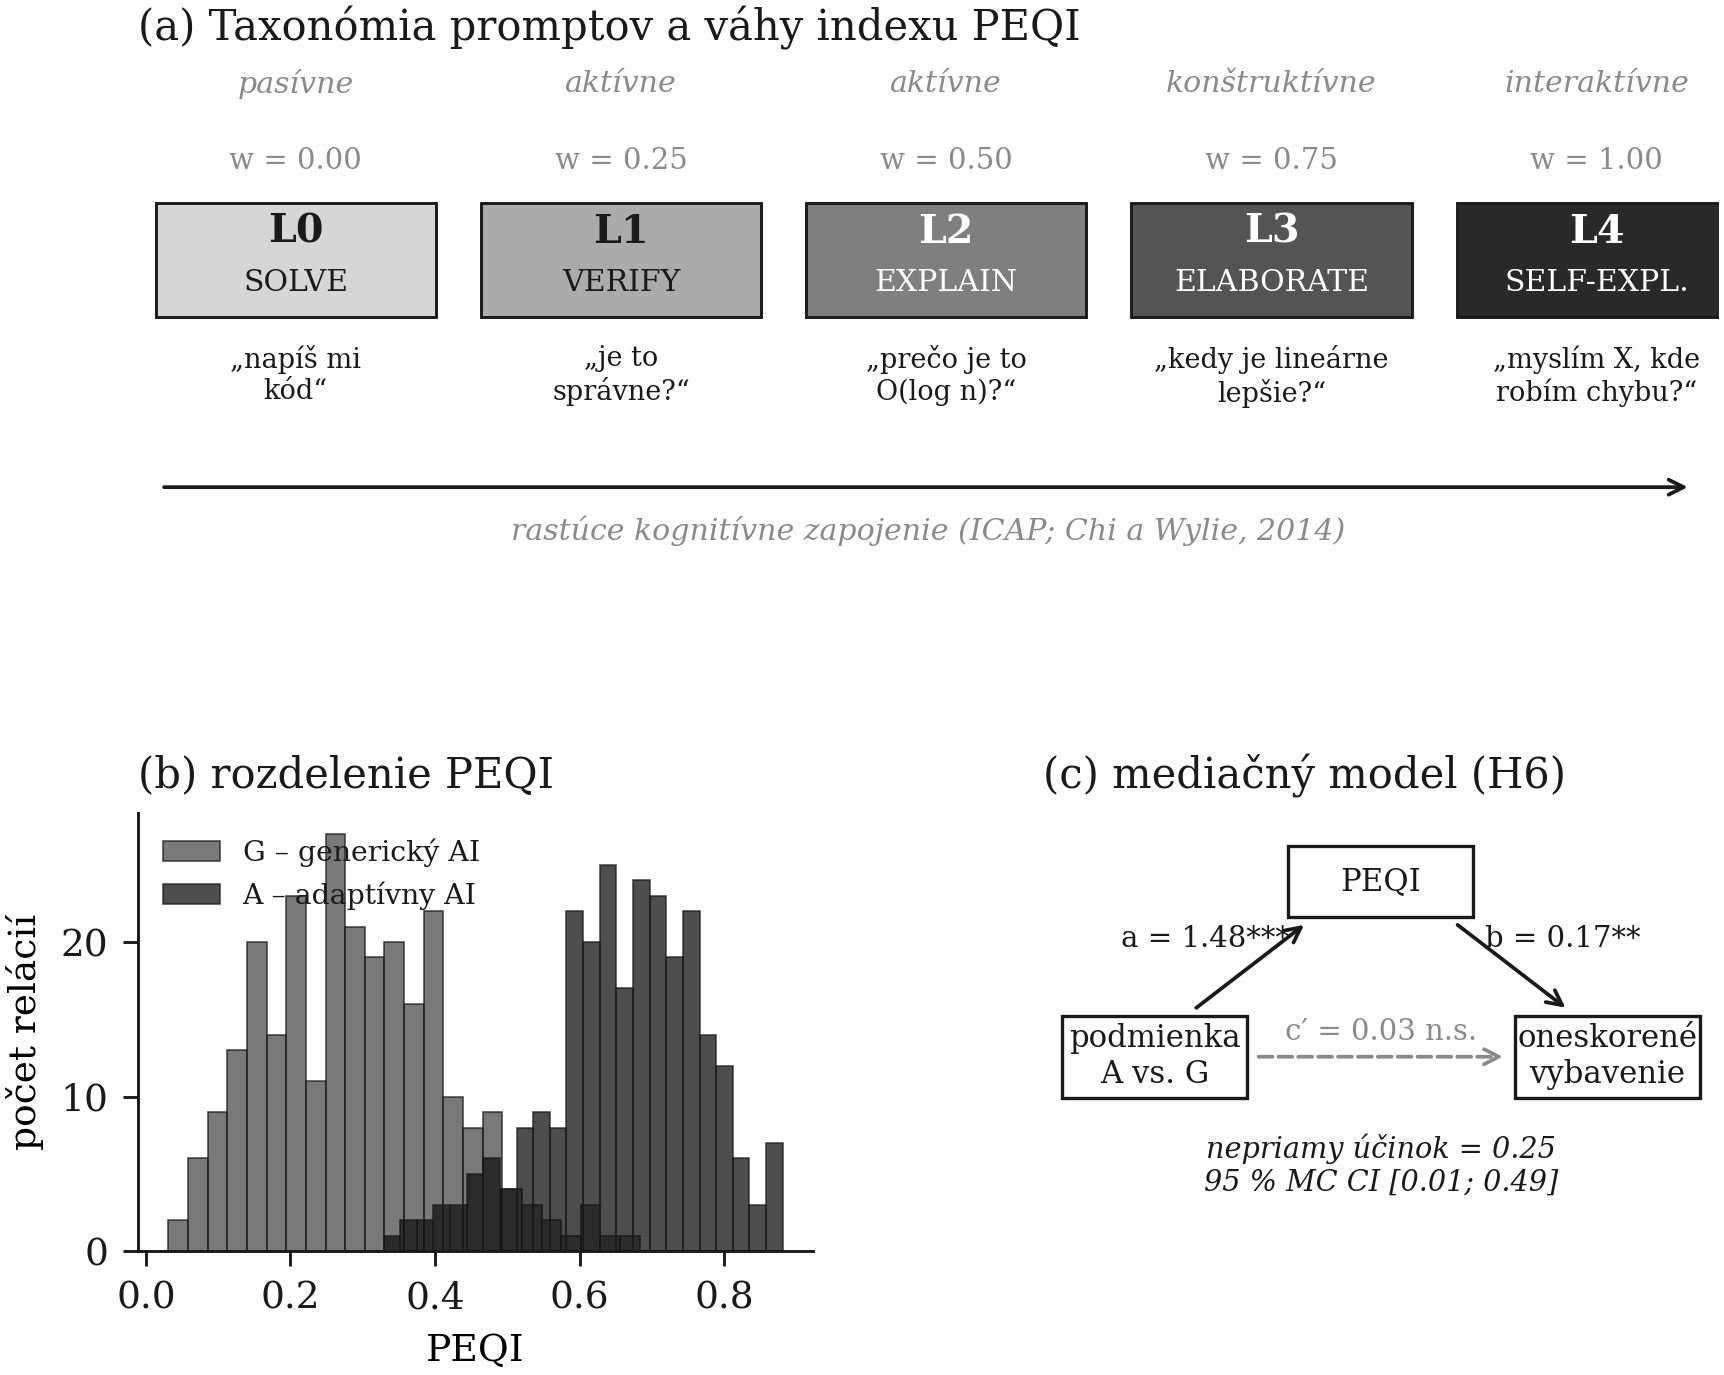
\includegraphics[width=\textwidth]{assets/images/fig_peqi.png}
    \caption{(a)~Taxonómia promptov ukotvená v rámci ICAP a váhy indexu. (b)~Rozdelenie PEQI v podmienkach $G$ a $A$ na simulovaných dátach. (c)~Mediačný model H6 s odhadmi zo simulačnej validácie.}
    \label{fig:peqi}
\end{figure}

Index sa počíta ako vážený priemer cez prompty vzťahujúce sa k úlohe:
\begin{equation}
    \mathrm{PEQI} = \frac{1}{n_{\text{na tému}}}\sum_{i=1}^{n_{\text{na tému}}} w(\ell_i),
    \qquad w = (0{,}00;\ 0{,}25;\ 0{,}50;\ 0{,}75;\ 1{,}00)
    \label{eq:peqi}
\end{equation}
pre úrovne $L_0$ až $L_4$; prompty zaradené ako \emph{mimo tému} sa z menovateľa vylučujú. Doplnkovo vykazujeme mieru offloadingu $\mathrm{OR}=(n_{L_0}+n_{L_1})/n_{\text{na tému}}$, ktorá je ľahšie interpretovateľná pre školskú prax.

Voľba rovnomerných váh je arbitrárna, a preto je nutné overiť, či od nej nezávisia závery. V citlivostnej analýze prepočítavame index s alternatívnym vážením $(0{,}0;\,0{,}2;\,0{,}4;\,0{,}7;\,1{,}0)$ a s čisto ordinálnou verziou (mediánová úroveň). Na simulovaných dátach sa PEQI zmení o menej než $0{,}03$ a poradie podmienok zostáva zachované. Toto však overuje len necitlivosť na \emph{monotónne} preváženie; teoreticky spornú otázku~--- či najvyššia úroveň vôbec zaslúži prémiu~--- overuje až analýza v časti~\ref{sec:icap-rung}.

\subsection{Sporný najvyšší stupienok a čo z neho index potrebuje}
\label{sec:icap-rung}

Váha $1{,}00$ pre úroveň $L_4$ nie je návrhové rozhodnutie, ale prevzaté tvrdenie: že \emph{interaktívne} zapojenie prináša viac než \emph{konštruktívne}. Toto tvrdenie je najslabšie podloženým miestom celého rámca a práca by naň nemala stavať bez výhrady.

\paragraph{Prečo je sporné.} Thurn a kolektív~\cite{thurn2023icapcritique} upozorňujú, že systematické overenie hierarchie $I>C>A>P$ neexistuje a že samotní autori rámca uvádzajú svoj prehľad dôkazov ako \emph{selektívny}. V štúdii, ktorú Chi predkladá ako najsilnejší test hierarchie~\cite{menekse2013dola}, bol podľa nich rozdiel medzi interaktívnym a konštruktívnym režimom zanedbateľný a nevýznamný. Najväčšia terénna štúdia rámca~\cite{chi2018translating} potvrdila $C>A$, ale vzťah $I>C$ netestovala: v triedach zamýšľaných ako interaktívne sa ku kolaboratívnej spolutvorbe vzťahovalo len 7\,\% zadaní, takže podmienka vznikla len na papieri.

\paragraph{Prečo je sporný dvojnásobne pri stroji.} Chi definuje interaktívny režim dvoma podmienkami: obaja partneri musia prispievať generatívne a ich príspevky sa musia navzájom rozvíjať, pričom ziskom má byť poznatok, \emph{ktorý by ani jeden z partnerov sám nevytvoril}~\cite{chi2018translating}. Pri jazykovom modeli taká veličina neexistuje~--- model vie vytvoriť celé riešenie sám. Chýba aj druhý mechanizmus, na ktorom rovesnícky dialóg stojí: partner, ktorý nerozumie a vynúti si preformulovanie. Model spravidla nerozumie zle a vždy signalizuje porozumenie, takže slučka opravy sa nespustí. Existujú návrhy, ktoré tento nedostatok riešia tým, že modelu \emph{zámerne} vložia chybu a žiak ju diagnostikuje~\cite{kucharavy2025proteges}; táto práca taký návrh netestuje a uvádza ho medzi ďalším postupom.

\paragraph{Čo z toho index potrebuje.} Úroveň $L_4$ v tejto taxonómii nie je Chiho interaktívny režim. Kóduje sa \emph{jediná} žiacka výpoveď, nie dyáda, takže $L_4$ je podľa Chiho vlastných kritérií \emph{konštruktívny úkon adresovaný partnerovi}~--- predpoklad interaktivity, nie jej doklad. Poctivý opis škály preto znie: gradient konštruktívneho zapojenia, usporiadaný podľa toho, koľko kognitívneho úkonu si žiak ponechá, s $L_4$ ako bodom, v ktorom sa jeho vlastná konštrukcia stáva dostupnou pre cudziu kritiku. Také usporiadanie vyžaduje len $C>A>P$ a gradient \emph{vnútri} konštruktívneho pásma. Nevyžaduje $I>C$.

\paragraph{Overenie, že závery od sporného stupienka nezávisia.} Index prepočítavame štyrmi váženiami: pôvodným, \emph{plochým} ($L_4$ dostane rovnakú váhu ako $L_3$), \emph{znevýhodňujúcim} ($L_4$ dostane menej než $L_3$~--- verzia, v ktorej dialóg so strojom nahrádza vlastné uvažovanie) a ordinálnym. Rozdiel $A-G$ zostáva kladný a významný pri všetkých štyroch a mení sa z \icapGapStd{} na \icapGapFlat, \icapGapDem{} a \icapGapOrd. Sporný stupienok nesie len \icapRungShare\,\% rozdielu medzi podmienkami; zvyšných \icapRestShare\,\% pochádza zo \emph{spodku} škály~--- podmienka $G$ vyvoláva prompty úrovní $L_0$ a $L_1$, ktoré podmienka $A$ nevyvoláva. Index teda oddeľuje podmienky podľa toho, koľkému offloadingu zabráni, nie podľa toho, koľko spolutvorby vytvorí.

Stojí za poznámku, že práve v tejto štúdii je sporná úroveň neobvykle častá: v podmienke $A$ tvorí \icapLfourA\,\% promptov k téme oproti \icapLfourG\,\% v podmienke $G$. V bežnom používaní je zriedkavá~--- rozbor 784~interakcií žiakov s konverzačným nástrojom nachádza prevahu pasívnych a aktívnych otázok~--- ale adaptívna vrstva je navrhnutá tak, aby ju vyvolávala. Neistá váha teda zaťažuje práve to miesto, kam manipulácia tlačí, čo je najnepriaznivejší možný prípad a ďalší dôvod, prečo sa na ňu neoprieť.

\paragraph{Vopred stanovený dyadický test.} Spor sa dá rozhodnúť dátami tejto štúdie a preto ho preregistrujeme. Ku každému promptu sa doplnkovo nakóduje \emph{odpoveď} asistenta (generatívna alebo nie) a \emph{nasledujúci} prompt žiaka (rozvíja odpoveď alebo nie). Z toho vznikne ukazovateľ skutočnej interaktivity podľa oboch Chiho kritérií. Testuje sa, či pridá prediktívnu hodnotu nad rámec PEQI. Ak áno, najvyšší stupienok si svoju váhu v tomto prostredí zaslúži. Ak nie, interaktívna úroveň ICAP pri strojovom partnerovi nerobí nič~--- a to je zistenie, ktoré stojí za vykázanie samo osebe.

\subsection{Kódovanie a jeho spoľahlivosť}

Kódovanie prebieha v troch krokoch. \emph{Po prvé}, dvaja nezávislí kódovatelia nakódujú ručne kotviaci súbor a náhodne vybraných 20\,\% všetkých promptov; vykazuje sa Krippendorffova $\alpha$~\cite{krippendorff2004content} s prijateľnou hranicou $\alpha\geq0{,}80$ a Cohenova $\kappa$~\cite{landis1977kappa}. \emph{Po druhé}, na ručne nakódovanom súbore sa natrénuje automatický klasifikátor. \emph{Po tretie}, klasifikátor sa validuje oproti zadržanej časti ručných kódov; ak dosiahne $\kappa\geq0{,}75$, použije sa na zvyšok korpusu, inak sa kóduje ručne celý korpus.

Klasifikátor je zámerne postavený na priehľadných lexikálnych a štruktúrnych príznakoch (prítomnosť žiadosti o artefakt, prítomnosť vlastnej hypotézy, prítomnosť porovnávacej formulácie, dĺžka, prítomnosť kódu) a multinomickej logistickej regresii, nie na neinterpretovateľnom modeli. Dôvod je praktický: škola aj oponent musia vedieť overiť, \emph{prečo} bol konkrétny prompt zaradený tak, ako bol. Na kotviacom súbore 90~promptov dosahuje samotné rozhodovacie pravidlo $\kappa=\peqiRuleKappa$ a regresia v päťnásobnej krížovej validácii $\kappa=\peqiCvKappa$, pričom \peqiAdjacent\,\% chýb je posun o jedinú susednú úroveň~--- teda presne ten typ chyby, ktorý pri ordinálnej škále vedie k útlmu, nie k skresleniu smeru účinku.

\subsection{Doplnkové procesné ukazovatele}

PEQI opisuje \emph{obsah} interakcie. Dopĺňame ho o tri ukazovatele jej \emph{priebehu}, ktoré sú odvoditeľné z časových značiek a zo zadaných odpovedí:

\begin{description}[leftmargin=1.9cm, style=nextline, nosep]
    \item[$T_1$] čas od zobrazenia úlohy po prvý prompt. Krátky čas znamená, že žiak úlohu ani neprečítal, kým delegoval.
    \item[ABHR] podiel úloh, pri ktorých žiak urobil vlastný pokus pred prvým promptom. Priamo operacionalizuje rozlíšenie medzi žiadaním pomoci a vyhýbaním sa úsiliu~\cite{aleven2003help,baker2004gaming}.
    \item[VTR] podiel doslovného prevzatia textu asistenta do odovzdanej odpovede, počítaný ako normalizovaná dĺžka najdlhšej spoločnej podpostupnosti. Meria kopírovanie bez spracovania.
\end{description}

\section{Učiteľská vetva}
\label{sec:ucitelia}

Zadanie žiada vyhodnotiť dopady na študentov \emph{či} učiteľov. Práca sa sústreďuje na žiakov, no učiteľská vetva sa dopĺňa z troch dôvodov, z ktorých ani jeden nie je formálny.

\emph{Po prvé}, učiteľ je ten, kto o zavedení rozhoduje. Zistenie, že adaptívna vrstva funguje lepšie než generický nástroj, nemá nijaký účinok, ak ju učiteľ nepoužije~--- a doložené nasadenia ukazujú, že nízke skutočné využitie je hlavným obmedzujúcim faktorom (časť~\ref{sec:nasadenie}).

\emph{Po druhé}, slovenský kontext robí túto vetvu obzvlášť informatívnou. Nástroje používa drvivá väčšina žiakov, kým vo vyučovaní ich používa približne štvrtina učiteľov a metodickú prípravu absolvovala necelá tretina (časť~\ref{sec:slovensko}). Štúdia, ktorá by merala len žiakov, by opísala jednu stranu rozdielu, ktorý je sám predmetom záujmu.

\emph{Po tretie}, je to lacné. Učitelia sú v miestnosti tak či tak a vedú všetky tri podmienky; ich pozorovania sú dostupné bez ďalšej organizácie.

\subsection{Čo sa zbiera}

\begin{table}[H]
\centering
\caption{Učiteľská vetva: nástroje a časovanie}
\label{tab:ucitelia}
\small
\begin{tabularx}{\textwidth}{@{}l l X@{}}
\toprule
\textbf{Kedy} & \textbf{Nástroj} & \textbf{Čo zisťuje} \\
\midrule
pred zberom & dotazník (12~položiek, 8~min) & doterajšie používanie nástrojov, absolvovaná príprava, očakávania od každej z troch podmienok \\
po každom bloku & kontrolný list vernosti & čo sa odchýlilo od scenára a prečo~--- slúži ako kontrola kvality \emph{aj} ako kvalitatívny údaj \\
po zbere & dotazník (10~položiek, 6~min) & čo pozoroval, ktorú podmienku by zaviedol, čo by zmenil \\
po zbere & pološtruktúrovaný rozhovor so 6~učiteľmi & prečo; vybraní podľa rozdielu medzi očakávaním a pozorovaním \\
\bottomrule
\end{tabularx}
\end{table}

\paragraph{Očakávanie pred a pozorovanie po.} Dotazník sa pýta na očakávaný účinok každej podmienky \emph{pred} zberom a na pozorovaný \emph{po} ňom. Rozdiel medzi nimi je samostatný údaj: učiteľ, ktorý čakal, že generický nástroj pomôže, a pozoroval opak, je informatívnejší prípad než učiteľ, ktorý mal pravdu. Výber šiestich učiteľov na rozhovor je stratifikovaný práve podľa veľkosti a smeru tohto rozdielu, nie podľa dostupnosti.

\paragraph{Prečo sa vernosť používa dvakrát.} Kontrolný list vernosti vznikol ako nástroj kontroly kvality: sleduje, či blok prebehol podľa scenára. Poznámky učiteľa o tom, čo sa pokazilo a prečo, sú však zároveň kvalitatívnym údajom o tom, čo nasadenie v slovenskej triede obnáša~--- a získavajú sa bez akejkoľvek ďalšej záťaže. Vykazujú sa súhrnne, nikdy nie tak, aby bolo možné identifikovať konkrétneho učiteľa alebo školu.

\subsection{Čo sa z učiteľskej vetvy tvrdiť nedá}

Osemnásť učiteľov nie je vzorka, z ktorej možno robiť kvantitatívne tvrdenia o slovenskom učiteľstve. Vetva je \emph{opisná} a vstupuje do práce ako kvalitatívny doplnok a ako vysvetlenie prípadných odchýlok v žiackych dátach, nie ako konfirmačné rameno. Učitelia navyše nie sú zaslepení voči podmienke~--- zaslepiť ich nemožno, lebo každú vedú~--- takže ich očakávania sú potenciálnym zdrojom očakávacieho efektu. Práve preto sú ich očakávania \emph{merané}: ak sa veľkosť účinku v triede sústavne mení s očakávaním učiteľa, je to zistenie, ktoré treba vykázať, a nie šum, ktorý treba stratiť.


\section{Priebeh zberu údajov}
\label{sec:priebeh}

\begin{description}[leftmargin=2.2cm, style=nextline, nosep]
    \item[T0a, týždeň 0] (\mplMinToa~min z jednej hodiny) Informovaný súhlas, ICAR (\mplGfItems{} položiek), iBobor (8~úloh).
    \item[T0b, týždeň 0] (\mplMinTob~min doma) Jr.~MAI a vstupný dotazník o doterajšom používaní nástrojov umelej inteligencie a o programátorskej skúsenosti, zadané cez EduPage. Dotazník o návykoch nie je test a nepotrebuje dozor; tým prestáva súťažiť o vyučovaciu hodinu s nástrojmi, ktoré merajú na čas.
    \item[P1--P3, týždne 1--3] (90~min týždenne) Vyučovací blok podľa priradenej sekvencie, bezprostredne po ňom okamžitý test s položkovou sebadôverou a krátky dotazník (záťaž podľa Leppinka, pocit naučenia, spokojnosť, vnímaná novosť formátu). Päťpoložkový predtest k danej téme sa zadáva na konci predchádzajúcej hodiny informatiky, pretože v~bloku na neho nie je miesto (časť~\ref{sec:hodnotenie-ziakov}).
    \item[T4a a T4b, týždeň 6] (3 vyučovacie hodiny) Odložený test zo všetkých troch tém s~prestávkami medzi nimi, opakovaný ICAR ako negatívna kontrola (T4a), a v~samostatnej hodine transferový test a záverečný dotazník postojov (T4b). Rozdelenie je nutné: spolu je to 92~minút merania a najdlhší nepretržitý úsek by prekročil únavový strop. Termín nie je žiakom vopred oznámený a v medziobdobí sa témy zámerne neopakujú.
    \item[T5, týždeň 7] Polostrukturované rozhovory s 18~žiakmi vybranými stratifikovane podľa tercilu indexu PEQI. Rozhovor sa vedie nad \emph{vlastnými promptami} žiaka, ktoré sa mu ukážu, nie nad spomienkou na hodinu. Úplný protokol vrátane desiatich otázok a pravidiel analýzy je v prílohe~\ref{sec:rozhovory}. Vykonateľný protokol celého zberu pre slovenskú školu~--- minútový rozpis, role, toky údajov, súhlasy a postup pri zlyhaniach~--- je v prílohe~\ref{chapter:protokol}.
\end{description}

Trojtýždňový odstup medzi poslednou lekciou a odloženým testom je zvolený zámerne. Je dosť dlhý na to, aby sa krivky zabúdania jednotlivých podmienok stihli rozísť, a dosť krátky na to, aby sa zmestil do jedného školského polroka. Neoznámenie termínu bráni tomu, aby sa meralo opakovanie namiesto retencie.

\paragraph{Testovací efekt.} Samotné absolvovanie okamžitého testu posilňuje neskoršie vybavenie~\cite{roediger2006test}. Tento efekt je prítomný vo všetkých podmienkach rovnako, a preto neskresľuje \emph{kontrast} medzi nimi; zvyšuje však absolútnu úroveň odloženého výkonu.

Doteraz to bola kvalitatívna poznámka. Teraz je vyčíslená, a je väčšia, než sa dalo tušiť. Kotviace položky sú v~oboch formách totožné, takže žiak ich v~odloženom teste vidí druhýkrát a ich druhé zodpovedanie je vybavovacie precvičenie. Pri precvičení $0{,}25$~logitu sa vložené zabúdanie \asmEqPlanted{} odhadne na \asmTeForgetting{}~--- teda takmer celé zmizne. Kontrast medzi podmienkami chránený \emph{je}: odhadne sa na \asmTeContrast{} pri vloženom \asmTeContrastPlanted{}. Konfirmačná rodina je teda v~poriadku a absolútna úroveň zadržania nie, čo uvádzame ako priznané obmedzenie. Rotovaný dizajn, ktorý veľkosť precvičenia \emph{identifikuje} náhodným pridelením namiesto toho, aby ju predpokladal, je navrhnutý a overený v~prílohe~\ref{chapter:hodnotiaci-modul}, časti~\ref{sec:rotovane-kotvenie}; čaká na pilot a do primárneho dizajnu tejto práce nevstupuje.

\section{Ako nástroj overuje a vyhodnocuje žiakov}
\label{sec:hodnotenie-ziakov}

Doterajšie časti povedali, \emph{čo} sa meria a \emph{prečo}. Táto hovorí, čím~--- teda ako sa meranie na žiakovi skutočne vykoná, skóruje, skontroluje a vráti. Úplný opis je v~prílohe~\ref{chapter:hodnotiaci-modul}; tu je šesť rozhodnutí, bez ktorých by zostala metodika návrhom a nie vykonateľným postupom.

\paragraph{Položka je údaj, nie próza.} Merací nástroj existoval doteraz práve raz, ako text prílohy. To stačí na jeho zdokumentovanie a nestačí na administrovanie, takže by musela vzniknúť druhá kópia~--- tá, ktorú žiak vidí. Dve kópie jednej špecifikácie sa rozídu; v~tejto práci sa to už dvakrát stalo a oba razy sa oprava dostala len do jednej z~nich. Položky preto žijú v~zásobníku (\asmBanks{}~nástrojov, \asmItems{}~položiek), z~ktorého ich berie aj program, čo ich administruje, aj ten, čo ich skóruje, aj príloha, ktorá ich tlačí. Validátor zásobníka odmietne okrem iného položku bez kľúča, rozptyľovač bez diagnózy, formu nesediacu na špecifikačnú tabuľku a kotviacu položku, ktorá nie je v~oboch formách totožná.

\paragraph{Žiaka treba spoznať päťkrát a nesmie sa dať pomenovať.} Primárny výstup je zmena, takže treba spojiť päť príležitostí jednej osoby; ochrana žiaka zakazuje výskumníkovi tú osobu poznať. Protokol to riešil školou drženým zoznamom kódov a prvú polovicu~--- že žiak ten kód zadá správne~--- nechával na jeho prsty. Pri 330~žiakoch sa kód píše asi 1\,650-krát, a preklep nevyrobí chybu, ale dve: jeden žiak ticho stratí príležitosť, a žiak, ktorý neexistuje, ticho získa riadok. Kód má preto kontrolný znak, abecedu bez zámeniteľných znakov a pravidlo „jeden kód, jedno sedenie“. Všetky jednoznakové preklepy a všetky prehodenia znakov sa zachytia \emph{pri klávesnici}, kým je žiak v~triede.

\paragraph{Úsilie pri teste sa meria, nie predpokladá.} „Žiaci sa naučili viac“ a „žiaci sa viac snažili na teste po hodine, ktorá ich bavila“ sú ten istý kontrast, pokiaľ ich niečo neoddelí. Negatívna kontrola povie, že je niečo zlé, nie čo; úsilie sa dá merať priamo z~časov jednotlivých položiek. Rozdiel v~úsilí $0{,}08$~--- taký, ktorý by vedel predstierať najmenší zaujímavý účinok~--- sa odhalí v~\asmEffortDetect{} prípadov pri falošnej pozitivite \asmEffortFalsePos{}. Papierový test toto číslo nevyrobí vôbec, a je to najsilnejší jediný argument pre digitálnu administráciu.

\paragraph{Kontaminácia testu je meranie, nie dozor.} Toto je štúdia o~vplyve nástroja umelej inteligencie na učenie a jej výstupom je test, ktorý žiak píše s~telefónom v~kapse. Doterajšou odpoveďou bola položka V12 kontrolného listu~--- tvrdenie dozorcu o~dvadsiatich obrazovkách. Nástroj namiesto toho zaznamenáva päť rodín príznakov z~troch nezávislých zdrojov, vylúči odpoveď len pri dvoch príznakoch z~\emph{rôznych} rodín, a je kalibrovaný na stretnutí T0a, kde kontaminácia nie je možná: čokoľvek tam označí, je falošná pozitivita konštrukciou. Pri realistickom nazeraní zachytí \asmIntegDetect{} kontaminovaných žiakov pri falošnej pozitivite \asmIntegFalsePos{}. Žiadny žiak sa škole nepomenuje~--- príznak, ktorý by sa mohol dotknúť známky, by zmenil motiváciu písať test poctivo a zničil by meranie, pre ktoré bol zavedený.

\paragraph{Kategorizácia, ktorú vie použiť aj jedna trieda.} Latentná profilová analýza (časť~\ref{sec:kategorizacia}) je tvrdenie o~vzorke: potrebuje stovky žiakov a označenie jedného žiaka závisí od toho, kto je v~súbore s~ním. Učiteľ s~jednou triedou z~nej nedostane nič. Nástroj preto obsahuje aj deterministické pravidlo nad absolútnymi, vopred stanovenými hranicami, ktoré funguje pri $n=1$, dáva porovnateľné označenia v~rôznych školách a rokoch, a vie jednou vetou povedať, prečo bol žiak označený. Pri jednej triede (\asmNClass{}~žiakov) dosahuje zhodu s~vloženou pravdou \asmRuleAriClass{}, kým zmesový model nenájde žiadne profily; pri \asmNStudy{}~žiakoch je zmes lepšia (\asmLpaAriStudy{} oproti \asmRuleAriStudy{}). Nie sú to konkurenti: zmes je výskumná otázka o~populácii, pravidlo je to, čo dostane škola.

\paragraph{A niečo sa škole vracia.} Učiteľ dostane počty mylných predstáv po položkách~--- nie „jedenásť žiakov nemá bod“, ale „jedenásť žiakov si myslí, že zdvojnásobenie poľa zdvojnásobí počet krokov“~--- bez rozpisu podľa podmienky, pretože ten učiteľovi neslúži a vyrába bunky, z~ktorých sa dá prečítať jednotlivec. Škola dostane agregáty s~potlačením buniek pod piatimi žiakmi. Žiak nedostáva individuálne skóre, a to z~uvedeného dôvodu: spoľahlivosť týchto nástrojov unesie porovnanie skupín, nie výrok o~jednotlivcovi.

\section{Technická infraštruktúra zberu}
\label{sec:infrastruktura}

Procesné ukazovatele pochádzajú z nástroja vyvinutého v technickej časti práce. Architektúra po revízii opísanej v časti~\ref{sec:riesenie} pozostáva z troch vrstiev:

\begin{enumerate}[nosep]
    \item \textbf{Záchytná vrstva} (mitmproxy~\cite{mitmproxy}) terminuje TLS na školskom notebooku pomocou certifikačnej autority nainštalovanej výhradne na zariadeniach zapojených do štúdie. Doplnok filtruje požiadavky podľa zoznamu povolených adries a zapisuje zhodné požiadavky do súboru vo formáte JSON Lines.
    \item \textbf{Spracovateľská vrstva} (Java) číta tento súbor, vykonáva odstránenie osobných údajov, pseudonymizáciu identifikátora žiaka a výpočet procesných ukazovateľov vrátane PEQI.
    \item \textbf{Cvičné rozhranie} dodáva udalosti, ktoré v sieťovej prevádzke nie sú viditeľné: zobrazenie úlohy, stlačenie klávesy, odoslanie pokusu, odomknutie riešenia. Bez nich by nebolo možné počítať $T_1$ ani ABHR.
\end{enumerate}

\paragraph{Pokrytie a jeho meranie.} Nástroj zachytí len prevádzku zo školského zariadenia. Žiak môže použiť vlastný telefón, a taká interakcia zostane neviditeľná. Preto meriame \emph{mieru pokrytia}: podiel žiakov, ktorých počet zachytených promptov je konzistentný s počtom odoslaní zaznamenaných cvičným rozhraním. Nekonzistentné prípady označujeme a vykazujeme citlivostnú analýzu bez nich. Rovnaký mechanizmus slúži na detekciu \emph{kontaminácie}~--- prevádzka smerujúca na jazykový model počas podmienky $K$ je porušením protokolu a zakladá rozdiel medzi analýzou podľa pôvodného priradenia a analýzou podľa skutočného priebehu.

\section{Štatistický plán analýzy}
\label{sec:sap}

Plán je uzavretý pred zberom dát a spolu s kódom zaregistrovaný~\cite{nosek2018preregistration}. Úplné znenie vrátane spustiteľného kódu je v prílohe~\ref{chapter:sap}.

\subsection{Primárny model}

Primárnym ukazovateľom je Raschova miera odloženého vybavenia $\theta_{\mathrm{DRT}}$. Model je lineárny zmiešaný model so štruktúrou náhodných efektov zodpovedajúcou dizajnu~\cite{barr2013maximal,bates2015lme4}:
\begin{equation}
    \theta_{\mathrm{DRT}, ijk} = \beta_0 + \tau_{c[ijk]} + \pi_{p[ijk]} + \gamma_{q[ijk]}
    + \beta_1\theta_{\mathrm{pre},ij} + \beta_2 g_{f,ij} + u_k + v_{j(k)} + \varepsilon_{ijk}
    \label{eq:model}
\end{equation}
kde $\tau_c$ je účinok podmienky, $\pi_p$ účinok periódy, $\gamma_q$ prenos z predchádzajúcej periódy, $u_k$ náhodný intercept triedy a $v_{j(k)}$ náhodný intercept žiaka vnoreného v triede.

\paragraph{Kódovanie prenosu.} V trojperiódovom štvorci je samostatná úroveň „bez prenosu“ pre prvú periódu dokonale kolineárna s indikátorom prvej periódy, čo robí návrhovú maticu singulárnou. Štandardným riešením~\cite{senn2002crossover} je priradiť prvej perióde referenčnú úroveň podmienky, takže odhadnuteľné sú dva parametre prenosu voči referencii. Toto obmedzenie sme odhalili až pri spustení plánu na simulovaných dátach~--- ukážka toho, prečo má zmysel plán pred zberom dát skutočne spustiť, nielen napísať.

\subsection{Kontrasty, ekvivalencia a multiplicita}
\label{subsec:kontrasty}

Hlavné kontrasty ($A-K$, $A-G$, $G-K$) odhadujeme ako vnútroindividuálne rozdiely s klastrovo robustným odhadom rozptylu na úrovni tried a odkazujeme ich na $t$-rozdelenie s $J-1$ stupňami voľnosti, kde $J$ je počet tried. Táto voľba je pri malom počte klastrov konzervatívna, čo overujeme aj simuláciou: pri skutočnom nulovom rozdiele je podiel zamietnutí $0{,}040$ oproti nominálnym $0{,}05$.

Tvrdenie H3 o \emph{neprítomnosti} rozdielu medzi $G$ a $K$ testujeme dvoma jednostrannými testami~\cite{lakens2017tost} voči najmenšej zaujímavej veľkosti účinku $\mathrm{SESOI}=0{,}30$ smerodajnej odchýlky, stanovenej pred zberom dát; ekvivalencia sa vyhlási, ak 90\,\% interval spoľahlivosti pre rozdiel leží celý vnútri pásma $\pm0{,}30$. Zdôvodnenie tejto hodnoty a jej operačné dôsledky rozoberá časť~\ref{sec:sesoi}, pretože to isté číslo tu plní dve úlohy, ktoré ťahajú opačným smerom.

\label{subsec:multiplicita}
Konfirmačnú rodinu tvoria tri testy na odloženom teste: $A>K$ (H3a), $G\equiv K$ (H3b) a $A>G$ (H6a). Na ne aplikujeme Holmovu postupnosť~\cite{holm1979sequential}. Výber práve týchto troch je odôvodnený v časti~\ref{sec:rqhypotezy}: sú to jediné tvrdenia, ktoré sú súčasne identifikované randomizáciou a schopné zlyhať. Okamžitý test do rodiny nepatrí~--- slúži ako kontrola manipulácie a ako druhý bod disociácie, nie ako predmet tvrdenia práce.

Sekundárne ukazovatele (transfer, kalibrácia, záťaž, procesné premenné) sú korigované metódou kontroly miery falošných objavov~\cite{benjamini1995fdr} v rámci vlastnej rodiny. Exploratívne analýzy sú označené ako exploratívne a ich $p$-hodnoty sa neinterpretujú konfirmačne.

\paragraph{Úspech celej rodiny, nie jej najpohodlnejšej časti.} Pri plánovaní sily nevykazujeme len silu jednotlivých testov, ale aj pravdepodobnosť, že \emph{všetky tri} prejdú Holmovou korekciou súčasne. Práve tá zodpovedá výsledku, o ktorom práca argumentuje. Vykazovanie sily jednotlivých testov by ju systematicky nadhodnocovalo.

\subsection{Odôvodnenie hranice praktickej významnosti}
\label{sec:sesoi}

Hodnota $\mathrm{SESOI}=0{,}30$ plní v pláne dve úlohy, ktoré ťahajú opačným smerom, a preto si zaslúži odôvodnenie dôkladnejšie než jednu vetu.

\begin{description}[leftmargin=0.6cm, nosep]
    \item[\textbf{Pri teste nadradenosti}] ($A>K$) je veľká hranica \emph{konzervatívna}: štúdia je dimenzovaná len na účinky aspoň takej veľkosti a skutočný účinok $0{,}15$ prehliadne.
    \item[\textbf{Pri teste ekvivalencie}] ($G\equiv K$) je veľká hranica \emph{zhovievavá}: čím širšie pásmo, tým ľahšie sa dve podmienky vyhlásia za nerozlíšiteľné.
\end{description}

Číslo zvolené tak, aby bolo bezpečné pre prvú úlohu, je tým samým automaticky nebezpečné pre druhú. Toto je bod, v ktorom sa v literatúre o ekvivalenčných testoch chybuje najčastejšie.

\paragraph{Na akej škále je hranica vyslovená.} Bežné referenčné hodnoty pre vzdelávacie zásahy sú odvodené zo \emph{štandardizovaných} testov výkonu. Kraft~\cite{kraft2020effectsizes} z rozdelenia 1\,942 účinkov v 747~randomizovaných štúdiách navrhuje hranice: pod $0{,}05$ malý, $0{,}05$ až $0{,}20$ stredný, $0{,}20$ a viac \emph{veľký}, pričom medián celého rozdelenia je $0{,}10$ a štvrtina účinkov je nulová alebo záporná. Lortie-Forgues a Inglis~\cite{lortieforgues2019rarely} uvádzajú priemer $0{,}06$ naprieč 141~štúdiami financovanými IES a EEF. Na tejto škále by hranica $0{,}30$ bola o polovicu väčšia než prah, od ktorého sa celoškolský zásah považuje za veľký.

Táto práca však nemeria na tejto škále. Meria výskumníkom zostaveným, s učivom zosúladeným Raschovsky kalibrovaným testom o 12 až 16~položkách. Cheung a Slavin~\cite{cheung2016methodological} na 645~štúdiách ukazujú, že účinky na nástrojoch zostavených výskumníkom sú zhruba \emph{dvojnásobné} oproti nezávislým štandardizovaným meraniam, pri úzko zosúladených testoch až štvornásobné. Hranica $0{,}30$ na použitej škále teda zodpovedá približne $0{,}08$ až $0{,}15$ na škále štandardizovaného testu~--- čo leží vnútri Kraftovho stredného pásma.

Pôvodné zdôvodnenie~--- „zhruba tretina štandardného ročného prírastku“~--- bolo v tomto ohľade nepresné: normy ročného prírastku sú odvodené zo štandardizovaných testov, kým výsledok práce je proximálny. Dve škály sa v jedinej vete tichom zamieňali. Hodnota môže byť správna; uvedený dôvod správny nebol.

\paragraph{Čo má hranica odôvodniť.} Lakens a kolektív~\cite{lakens2018tosttutorial} zdôrazňujú, že SESOI odpovedá na \emph{normatívnu} otázku~--- nie „aký veľký je tento účinok“, ale „prečo by účinok menší než tento nemal význam“~--- a že hranica uvedená bez odôvodnenia je bezcenná. Prijímame ju z nákladovej úvahy: zavedenie generického nástroja do vyučovania má nezanedbateľné náklady na čas, zariadenia a prípravu učiteľov, a rozdiel menší než $0{,}30$ na použitej škále (teda okolo $0{,}10$ štandardizovane) by tieto náklady neospravedlnil ani neodôvodnil zmenu praxe. To je tvrdenie o rozhodnutí, ktoré škola robí, nie o štatistike, a ako také je napadnuteľné~--- preto ho uvádzame explicitne.

\paragraph{Čo hranica v skutočnosti kupuje.} Rozhodujúce nie je, ako sa hranica nazýva, ale s akou pravdepodobnosťou plán vyhlási ekvivalenciu pri rôznych skutočných rozdieloch. Tabuľka~\ref{tab:sesoi} to vyčísľuje na 3000~simulovaných štúdiách na bunku pri $J=18$.

\begin{table}[H]
\centering
\caption{Pravdepodobnosť vyhlásenia $G\equiv K$ podľa skutočného rozdielu a šírky pásma ($J=18$)}
\label{tab:sesoi}
\small
\begin{tabular}{@{}lccccc@{}}
\toprule
skutočný rozdiel $G-K$ & $\pm0{,}15$ & $\pm0{,}20$ & $\pm0{,}25$ & $\mathbf{\pm0{,}30}$ & $\pm0{,}40$ \\
\midrule
$0{,}00$ (pravá nula) & \eqTNullBFifteen & \eqTNullBTwenty & \eqTNullBTwentyFive & \textbf{\eqTNullBThirty} & \eqTNullBForty \\
$0{,}10$ & \eqTTenBFifteen & \eqTTenBTwenty & \eqTTenBTwentyFive & \textbf{\eqTTenBThirty} & \eqTTenBForty \\
$0{,}15$ & \eqTFifteenBFifteen & \eqTFifteenBTwenty & \eqTFifteenBTwentyFive & \textbf{\eqTFifteenBThirty} & \eqTFifteenBForty \\
$0{,}20$ & \eqTTwentyBFifteen & \eqTTwentyBTwenty & \eqTTwentyBTwentyFive & \textbf{\eqTTwentyBThirty} & \eqTTwentyBForty \\
$0{,}25$ & \eqTTwentyFiveBFifteen & \eqTTwentyFiveBTwenty & \eqTTwentyFiveBTwentyFive & \textbf{\eqTTwentyFiveBThirty} & \eqTTwentyFiveBForty \\
\bottomrule
\end{tabular}
\end{table}

Riadok pre skutočný rozdiel $0{,}20$ je ten, ktorý je práca čitateľovi dlžná. Pri plánovanej hranici a plánovanej vzorke sa rozdiel tejto veľkosti vyhlási za „žiadny rozdiel“ v \eqTTwentyBThirty{} prípadov, teda zhruba raz z troch. Pri rozdiele $0{,}15$ je to \eqTFifteenBThirty. Nejde o chybu metódy TOST; je to presne to, čo hranica $0{,}30$ znamená, vyjadrené v jediných zmysluplných pojmoch.

\paragraph{Prečo hranicu nezužujeme.} Zúženie je možné a jeho cena je vyčíslená. Aby sa pri \emph{skutočnej nule} vyhlásila ekvivalencia v 80\,\% prípadov, je pri hranici $\pm0{,}30$ potrebných \eqClassesThirty{} tried, pri $\pm0{,}20$ už \eqClassesTwenty{} a pri $\pm0{,}15$ \eqClassesFifteen. Zúženie hranice na polovicu teda zdvojnásobuje štúdiu. Taký rozsah táto práca nemá k dispozícii a povedať to priamo je poctivejšie než zvoliť hranicu podľa toho, čo sa do vzorky zmestí.

\paragraph{Dôsledok pre formuláciu záveru.} Z toho plynie záväzné pravidlo, ktoré dopĺňame do plánu analýzy: záver z testu ekvivalencie sa nikdy neformuluje ako „$G$ je ekvivalentné $K$“, ale vždy ako „\emph{rozdiel väčší než $0{,}30$ smerodajnej odchýlky na použitej škále možno vylúčiť}“. Obe vety sú o tých istých dátach; len druhá je pravdivá. Spolu so záverom sa vykazuje aj tabuľka~\ref{tab:sesoi}, aby čitateľ videl, čo pásmo prepúšťa.

\subsection{Chýbajúce údaje}
\label{subsec:chybajuce}

Zmiešaný model využíva všetky dostupné pozorovania a je nezaujatý za predpokladu náhodného výpadku podmieneného modelovanými premennými (MAR). Tento predpoklad \emph{neoveriteľný nie je}~--- overiteľná je aspoň jeho slabšia verzia. Porovnávame vstupné charakteristiky žiakov s kompletnými a nekompletnými dátami a testujeme, či výpadok súvisí so vstupnými vedomosťami. Očakávame, že áno: slabší žiaci chýbajú častejšie. To vylučuje úplnú náhodnosť výpadku (MCAR) a je dôvodom, prečo sú vstupné vedomosti \emph{v modeli}, a nie len vykázané v tabuľke.

Ako citlivostnú analýzu vykonávame viacnásobnú imputáciu~\cite{rubin1987imputation} (20 imputácií) a doplnkovo úmyselne nepriaznivý scenár, v ktorom sa chýbajúcim hodnotám v podmienke $A$ priradí najhorší a v podmienkach $K$ a $G$ najlepší pozorovaný kvartil. Nepriaznivý scenár nie je hodnoverný, a to je jeho zmysel: je to hranica toho, čo by výpadok mohol spôsobiť, ak by bol maximálne nepriaznivý pre hypotézu. Ak záver prežije aj ten, výpadok ho nevysvetľuje; ak neprežije, vykazujeme to ako obmedzenie a nie ako podrobnosť v prílohe.

\subsection{Robustnostné analýzy}

Vopred stanovujeme päť robustnostných analýz. Každá z nich je implementovaná a spustená (kapitola~\ref{chapter:vysledky}); plán, ktorý ich vymenuje a jednu z nich vykoná, je plán, ktorý nebol preskúšaný.

\begin{enumerate}[nosep]
    \item \textbf{Len prvá perióda.} Z podstaty imúnne voči prenosu, ale medziskupinové a na tretine dát. Nevýznamnosť v tejto analýze je očakávaná a nesmie sa zamieňať s neprítomnosťou účinku.
    \item \textbf{Vylúčenie hodín s vernosťou pod 90\,\%.} Ak je účinok po vylúčení \emph{väčší}, je to v súlade s tým, že nízka vernosť účinok riedi, a nie s tým, že ho vytvára.
    \item \textbf{Analýza podľa skutočného priebehu.} Vylúčenie žiakov, u ktorých sa počas kontrolnej podmienky zachytila komunikácia s asistentom. Rozdiel oproti analýze podľa pôvodného priradenia meria dosah kontaminácie.
    \item \textbf{Hrubá úspešnosť namiesto Raschovej miery.} Overuje, že záver nezávisí od psychometrického modelu.
    \item \textbf{Náhodný sklon podmienky podľa triedy.} Pripúšťa, že účinok sa medzi triedami líši, namiesto predpokladu, že je konštantný. Táto analýza navyše \emph{odhaduje} rozptyl $\tau^2_{ct}$~--- práve ten parameter, ktorý sa v analýze sily ukázal ako viazané obmedzenie. Plánovací predpoklad sa tým stáva overiteľným namiesto toho, aby zostal domnienkou.
\end{enumerate}

\section{Identifikácia mechanizmu: čo randomizácia dokáže a čo nie}
\label{sec:identifikacia}

Táto časť sa venuje najslabšiemu miestu celej práce. Pomenúvame ho, kvantifikujeme a ošetrujeme namiesto toho, aby sme ho obišli.

\subsection{Problém}

Dizajn randomizuje \emph{podmienku}, nie \emph{kvalitu promptov}. Z toho vyplýva rozdelenie, ktoré je pre interpretáciu zásadné (obrázok~\ref{fig:dag}~a):

\begin{itemize}[nosep]
    \item \textbf{Celkový účinok} podmienky $A$ oproti $G$ na odložené vybavenie je identifikovaný dizajnom. O tom niet sporu.
    \item \textbf{Dráha $a$}, teda účinok podmienky na PEQI, je identifikovaná dizajnom rovnako.
    \item \textbf{Dráha $b$}, teda účinok PEQI na odložené vybavenie, identifikovaná \emph{nie je}. Randomizácia nepovedala žiakovi, ako sa má pýtať; to je jeho správanie, a ako každé správanie je zamenené s tým, čo ho spôsobuje.
\end{itemize}

Mediačná analýza dráhu $b$ odhaduje, no jej odhad je nezaujatý len za predpokladu \emph{sekvenčnej ignorovateľnosti}~\cite{imai2010mediation}~--- neexistencie nepozorovanej spoločnej príčiny mediátora a výsledku. Tento predpoklad je v školskej triede takmer isto porušený. Svedomitosť pôsobí na to, či si žiak dá tú prácu a sformuluje vlastnú úvahu, aj na to, koľko si zapamätá. To isté platí pre záujem o predmet, rýchlosť čítania alebo domácu podporu. Práca, ktorá by uviedla nepriamy účinok a pokračovala ďalej, by tvrdila viac, než na čo má nárok. Bullock, Green a Ha~\cite{bullock2010mechanism} tento problém zhrnuli tak, že randomizácia intervencie o mechanizme nehovorí nič, a bežná prax, ktorá z randomizovaného experimentu odvodzuje mediáciu, zamieňa dve úplne rozdielne identifikačné situácie. Formálne podmienky identifikácie a ich hranice rozoberá VanderWeele~\cite{vanderweele2015explanation}; grafický jazyk, v ktorom je rozdiel medzi obrázkom~\ref{fig:dag}~a a bežnou mediačnou schémou viditeľný, pochádza od Pearla~\cite{pearl2009causality}.

\begin{figure}[H]
    \centering
    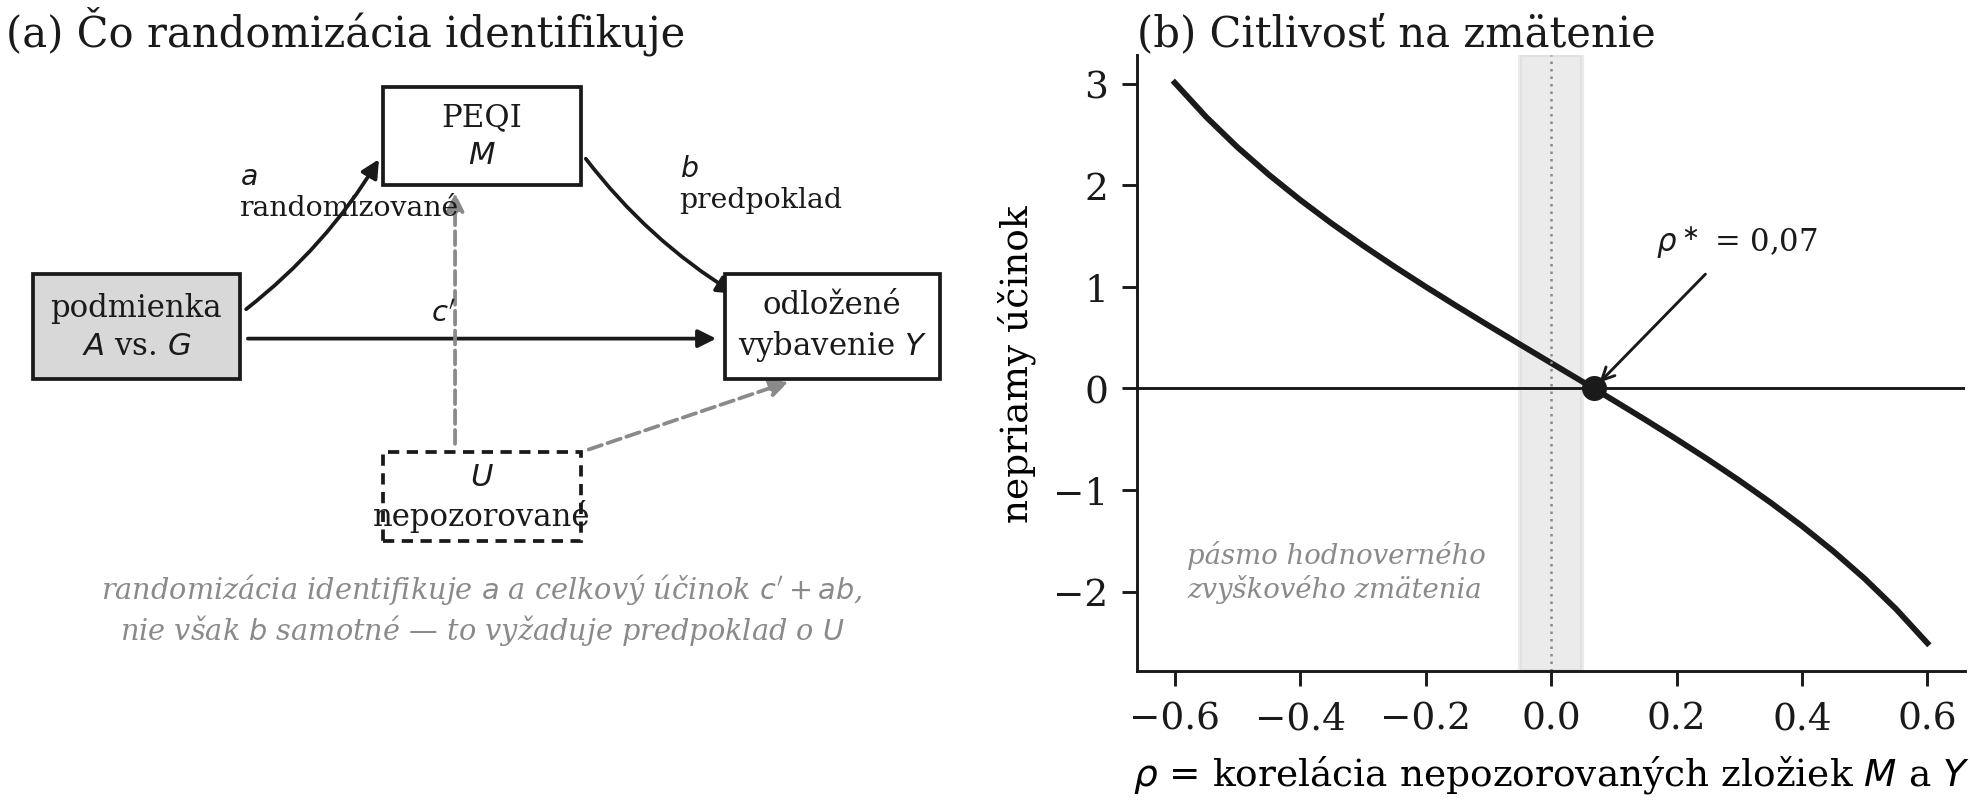
\includegraphics[width=\textwidth]{assets/images/fig_dag.png}
    \caption{(a)~Kauzálny graf. Randomizácia identifikuje dráhu $a$ a celkový účinok $c'+ab$; dráhu $b$ neidentifikuje, pretože nepozorovaná premenná $U$ môže pôsobiť na PEQI aj na vybavenie súčasne. (b)~Citlivosť nepriameho účinku na silu takého zmätenia; $\rho^\ast$ je hodnota, pri ktorej nepriamy účinok zaniká.}
    \label{fig:dag}
\end{figure}

\subsection{Triangulácia: tri odhady, tri rôzne predpoklady}
\label{sec:triangulacia}

Namiesto jedného odhadu s jedným nevysloveným predpokladom odhadujeme tú istú veličinu trikrát. Podstatné je, že predpoklady nie sú vnorené a porušujú ich rôzne veci: zhoda medzi odhadmi je preto dôkazom, a nezhoda lokalizuje, ktorý predpoklad zlyhal.

\begin{description}[leftmargin=0.6cm, nosep]
    \item[\textbf{(1) Mediačný model.}] Súčin koeficientov s Monte Carlo intervalom pre nepriamy účinok~\cite{preacher2012montecarlo}. \emph{Predpoklad:} sekvenčná ignorovateľnosť. Všetky tri rovnice používajú rovnakú množinu kontrolných premenných, a to výhradne predintervenčných, takže rozklad \emph{celkový $=$ priamy $+$ nepriamy} skutočne platí a podiel mediácie niečo znamená. Miešanie kontrolných množín~--- odhadnúť dráhu $b$ s pointervenčnou kontrolou a celkový účinok bez nej~--- dáva podiel mediácie nad jednotkou a je rozkladom ničoho.
    \item[\textbf{(2) Inštrumentálna premenná.}] Randomizovaná pedagogická vrstva sa použije ako \emph{inštrument} pre kvalitu promptov. \emph{Predpoklad:} podmienka pôsobí na odložené vybavenie \emph{výhradne} cez kvalitu promptov (podmienka vylúčenia). Tento predpoklad je iný než predpoklad (1) a porušujú ho iné veci~--- viď nižšie. Ide o štandardné použitie inštrumentálnej premennej v zmysle Angrista, Imbensa a Rubina~\cite{angrist1996iv}. Odhad je Waldov podiel redukovanej formy a prvého stupňa, so zhlukovo robustným rozptylom~\cite{cameron2015cluster} a s vykázanou $F$-štatistikou prvého stupňa; za slabý inštrument sa podľa zaužívaného kritéria považuje $F<10$~\cite{staiger1997weak}.
    \item[\textbf{(3) Dávková závislosť.}] Sklon PEQI k vybaveniu \emph{v rámci} samotnej podmienky $G$, kde o kvalite promptov rozhoduje žiak a nie manipulácia. \emph{Predpoklad:} žiadny nad rámec linearity; nič tu nie je identifikované. Uvádza sa preto, že jeho \emph{neprítomnosť} by bola poškodzujúca: ak by kvalita promptov nepredpovedala nič tam, kde ju dizajn nevynucoval, mechanizmové vysvetlenie by stálo výhradne na tom, že manipulácia zafungovala z nejakého iného dôvodu.
\end{description}

\paragraph{Prečo je podmienka vylúčenia v tomto dizajne hodnovernejšia než inde.} Podmienky $G$ a $A$ zdieľajú model, úlohy, rozhranie, učiteľa aj čas. Kanálov, ktorými by mohla pedagogická vrstva pôsobiť mimo kvality promptov, je preto málo a sú vymenovateľné. Sú dva: adaptívne poradie úloh riadené modelom znalostí, a brána vlastného vysvetlenia. Druhý z nich možno považovať za súčasť kvality interakcie~--- práve vynucuje akty typu L4~--- ale prvý nie. Podmienka vylúčenia je teda čiastočne porušená a odhad inštrumentálnou premennou je \emph{horná hranica} veľkosti dráhy $b$, ak ostatné kanály pôsobia rovnakým smerom. Uvádzame to takto a nie inak.

\paragraph{Čo do kontrolných premenných patrí a čo nie.} Okamžitý test je pointervenčná premenná. V odhade inštrumentálnou premennou preto medzi kontrolami \emph{nie je}~--- podmieňovanie pointervenčnou premennou by zablokovalo časť práve odhadovanej dráhy. V mediačnom modeli ho uvádzame osobitne ako doplnkovú, vecne motivovanú veličinu: dráhu $b$ „očistenú o okamžité učenie“, ktorá odpovedá na otázku, či kvalita promptov predpovedá to, čo \emph{prežije}, nad rámec toho, čo žiak vedel na konci hodiny. Táto hodnota sa nikdy nezlučuje s rozkladom celkového účinku.

\subsection{Analýza citlivosti}
\label{subsec:citlivost}

Zhoda troch odhadov nevylučuje, že všetky tri sú posunuté rovnakým smerom. Preto vyčísľujeme, aké silné by nepozorované zmätenie muselo byť.

Postup zodpovedá parametrizácii citlivosti podľa Imaia, Keeleho a Yamamota~\cite{imai2010sensitivity}. V lineárnom modeli $M = a\,T + \varepsilon_M$, $Y = c'\,T + b\,M + \varepsilon_Y$ s koreláciou $\rho = \mathrm{corr}(\varepsilon_M, \varepsilon_Y)$ platí, že regresia $Y$ na $(T, M)$ vracia
\begin{equation}
    \hat{b} = b + \rho\,\frac{\sigma_{\varepsilon_Y}}{\sigma_{\varepsilon_M}},
    \label{eq:sens}
\end{equation}
takže opravená dráha je $b(\rho) = \hat{b} - \rho\,s_{\mathrm{res}}\big/\big(\sqrt{1-\rho^2}\,s_M\big)$ a nepriamy účinok zaniká pri
\begin{equation}
    \rho^\ast = \frac{k}{\sqrt{1+k^2}}, \qquad k = \hat{b}\,\frac{s_M}{s_{\mathrm{res}}} .
\end{equation}

Interpretácia je priama a pre čitateľa zrozumiteľnejšia v podiele vysvetleného rozptylu: zmätenie, ktoré vysvetľuje podiel $R^2_M$ zvyškového rozptylu mediátora a $R^2_Y$ zvyškového rozptylu výsledku, vyvolá koreláciu $|\rho| = \sqrt{R^2_M R^2_Y}$. Hodnota $\rho^\ast$ teda hovorí, koľko nepozorovanej spoločnej príčiny by bolo treba na vysvetlenie celého zistenia.

\paragraph{Vopred stanovené rozhodovacie pravidlo.} Aby sa o sile dôkazu nerozhodovalo podľa toho, ako výsledok vyjde, stanovujeme pravidlo vopred. Ak $\rho^\ast \geq 0{,}30$, mechanizmové zistenie sa označuje za \emph{robustné}. Ak $\rho^\ast$ leží medzi $0{,}15$ a $0{,}30$, za \emph{podmienené} a v abstrakte sa uvádza spolu s touto výhradou. Ak $\rho^\ast < 0{,}15$, za \emph{krehké}: v takom prípade sa mechanizmové tvrdenie neuvádza medzi závermi práce, len medzi otvorenými otázkami. Hranicu $0{,}15$ volíme preto, že svedomitosť ako jediný nepozorovaný činiteľ hodnoverne vysvetlí okolo pätiny zvyškového rozptylu v oboch veličinách, čo zodpovedá $\rho \approx 0{,}2$.

\subsection{Sila a presnosť pre mechanizmus}

Pri mechanizme sú to dve rôzne otázky a zamieňajú sa. \emph{Sila} sa pýta, či bude odhad odlíšiteľný od nuly. \emph{Presnosť} sa pýta, či bude dosť úzky na to, aby k niečomu bol: interval od $0{,}02$ po $0{,}60$ vylučuje nulu a škole nepovie nič. Vopred preto stanovujeme kritérium presnosti: 95\,\% interval nie širší než $0{,}20$, čo je zhruba rozdiel medzi tvrdením „na kvalite promptov trochu záleží“ a „záleží na nej porovnateľne ako na samotnej hodine“.

\begin{figure}[H]
    \centering
    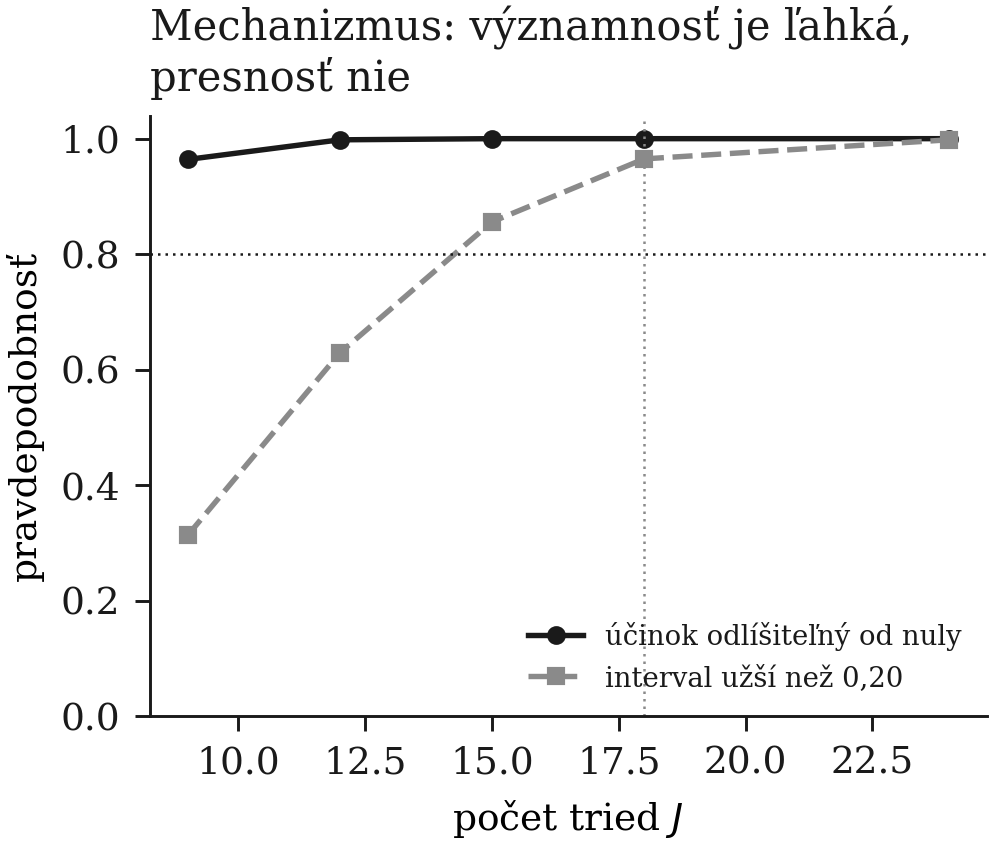
\includegraphics[width=0.62\textwidth]{assets/images/fig_mechanism.png}
    \caption{Sila a presnosť odhadu mechanizmu inštrumentálnou premennou. Odlíšiteľnosť od nuly je dosiahnutá už pri deviatich triedach; dostatočná presnosť nie.}
    \label{fig:mechanizmus}
\end{figure}

Výsledok je nesamozrejmý a posilňuje odporúčanie z časti~\ref{sec:sila} z úplne iného smeru. Pri deviatich triedach je pravdepodobnosť, že odhad bude významný, už $\powMechSignine$, ale pravdepodobnosť, že bude dosť presný, len $\powMechnine$. Pri 12~triedach je to $\powMechSigtwelve$ oproti $\powMechtwelve$ a až pri 18~triedach $\powMechSigeighteen$ oproti $\powMecheighteen$. Inými slovami: menšia vzorka by s vysokou pravdepodobnosťou priniesla mechanizmové zistenie, ktoré je štatisticky významné a prakticky nepoužiteľné. To je presne ten druh výsledku, ktorý sa publikuje a nikoho nikam neposunie.


\section{Diferenciálna chyba merania mediátora}
\label{sec:diferencialna}

Predchádzajúca časť sa pýtala, čo randomizácia o mechanizme dokáže preukázať. Celý ten výklad mlčky predpokladá, že PEQI je \emph{pozorovaná} veličina. Nie je. PEQI je \emph{odhadnutá} klasifikátorom a chyba toho odhadu nemusí byť nevinná, pretože môže závisieť práve od podmienky, ktorú dizajn randomizuje.

\subsection{Prečo tu chyba merania nie je len šum}

Podmienka $A$ obsahuje bránu sebavysvetlenia: vzorové riešenie sa neodomkne, kým žiak vlastnými slovami nenapíše, prečo si myslí, že jeho postup je správny, alebo kde si myslí, že urobil chybu (časť~\ref{sec:cvicne-rozhranie}). Rozhranie teda \emph{predpisuje} žiakom v podmienke $A$ jazykovú formu, ktorú v podmienke $G$ nič nevynucuje: „myslím si, že\ldots“, „podľa mňa\ldots“. Klasifikátor, ktorý túto formu číta ako doklad uvažovania, priradí promptom z podmienky $A$ systematicky vyššiu úroveň \emph{z dôvodu rozhrania}, nezávisle od toho, či za ňou nejaká úvaha naozaj stojí.

To nie je hypotetická obava. Prvá verzia klasifikátora v tejto práci priradila úroveň $L_4$ \emph{každému} z \venN{} kotviacich promptov úrovne $L_0$ a $L_1$, keď sa pred ne postavili štyri slová bez akéhokoľvek obsahu. Posun v priemernej váhe bol $\venDeltaBefore$ na prompt~--- viac než dvojnásobok celého medzipodmienkového rozdielu, na ktorý je štúdia dimenzovaná. Meranie tejto zraniteľnosti a jej odstránenie opisuje časť~\ref{sec:dominancia}; tu ide o to, čo by taká chyba spôsobila, keby sa neodstránila, a ako sa jej zvyšok dá ošetriť.

\subsection{Model chyby a tri tvrdenia}

Nech $A\in\{0,1\}$ je randomizovaná pedagogická vrstva, $M$ skutočná kvalita promptov, $Y$ retencia. Označme
\begin{align}
    M &= a\,A + u, & Y &= c'A + b\,M + \varepsilon, & \mathrm{cov}(u,\varepsilon) &= \sigma_{u\varepsilon},\\
    \widetilde{M} &= M + \delta\,A + e, & e &\perp (A, M, \varepsilon), & \mathrm{var}(e) &= \sigma_e^2 .
    \label{eq:mererr}
\end{align}
Parameter $\delta$ je \emph{diferenciálna} chyba~--- posun závislý od podmienky~--- kým $e$ je klasická, od podmienky nezávislá chyba. Spoľahlivosť $\widetilde{M}$ v rámci podmienky označme $\lambda = \mathrm{var}(u)/(\mathrm{var}(u)+\sigma_e^2)$.

Z rovníc~\eqref{eq:mererr} vyplývajú tri tvrdenia. Každé z nich je dvojriadkovým algebraickým dôsledkom a každé je zároveň overené simuláciou na štyristotisíc pozorovaniach v module \texttt{measurement.py}. Dôvod pre oba postupy naraz je ten, že algebru je ľahké urobiť správne na papieri a ľahké urobiť zle v kóde~--- a práca spúšťa kód.

\begin{description}[leftmargin=1.0cm, nosep]
    \item[\textbf{T1.}] \emph{Redukovaná forma je nedotknutá.} Odhad $\mathrm{cov}(Y,A)/\mathrm{var}(A) = c' + ab$ neobsahuje $\widetilde{M}$ vôbec, takže ho $\delta$ ani $e$ neovplyvnia. Pri platnosti vylučovacej podmienky ($c'=0$) je nepriamy účinok \emph{totožný} s redukovanou formou. Veličina „koľko z rozdielu medzi $A$ a $G$ prechádza cez kvalitu promptov“ je teda odolná voči \emph{ľubovoľne veľkej} chybe merania mediátora.
    \item[\textbf{T2.}] \emph{Inštrumentálny odhad je utlmený.} Platí $\hat\beta_{\mathrm{IV}} = \mathrm{ITT}_Y/(a+\delta) = b\cdot a/(a+\delta)$. Diferenciálna chyba nafúkne prvý stupeň, a tým \emph{zmenší} odhad účinku na jednotku. Smer je opačný, než naznačuje bežná intuícia, ktorá väčší prvý stupeň číta ako silnejšiu manipuláciu.
    \item[\textbf{T3.}] \emph{Mediačný odhad je najprv nafúknutý, potom utlmený.} Platí $\widehat{ab} = (a+\delta)\,\hat b$, kde $\hat b = (b\,\mathrm{var}(u) + \sigma_{u\varepsilon})/(\mathrm{var}(u)+\sigma_e^2)$. Pri nulovom zmätení mediátora s výsledkom je to $\mathrm{ITT}_Y\cdot(1+\delta/a)\cdot\lambda$.
\end{description}

\paragraph{Prípad presného zrušenia.} Z T3 vyplýva nepríjemný dôsledok. Pri $\delta/a = (1-\lambda)/\lambda$ sa obe skreslenia navzájom presne zrušia a mediačný odhad je nezaujatý~--- pričom \emph{každý} koeficient, z ktorého je zložený, je nesprávny. Pri hodnotách použitých v overovacej simulácii ($a=\measApath$, $\lambda=\measLambda$) k tomu dôjde pri $\delta = \measCancel$. Žiadna diagnostika postavená na bodovom odhade nevie tento prípad odlíšiť od bezchybného merania. Odlíšiť ho vie jedine audit.

\subsection{Dôsledok: kalibrovaná triangulácia}

Podiel oboch odhadov je
\begin{equation}
    \frac{\widehat{ab}_{\text{mediácia}}}{\widehat{ab}_{\mathrm{IV}}} = \Big(1+\frac{\delta}{a}\Big)\,\lambda ,
    \label{eq:ratio}
\end{equation}
a \emph{obe} veličiny na pravej strane sú odhadnuteľné: $\lambda$ zo štúdie spoľahlivosti, $\delta$ z auditu opísaného nižšie. Triangulácia z časti~\ref{sec:triangulacia} tým dostáva kalibrované očakávanie namiesto odhadu okom. Rozdiel medzi odhadmi väčší, než predpovedá~\eqref{eq:ratio}, nie je chyba merania; je to práve to zmätenie mediátora s výsledkom, ktoré ohraničuje $\rho^\ast$. V simulácii s $\rho=0{,}35$ podiel vyskočí z predpovedaných $\measRatioPred$ na $\measRatioConf$, čo je posun, ktorý sa na dátach dá uvidieť.

\paragraph{Čo z toho plynie pre vykazovanie.} Z T1 vyplýva poradie, v akom sa mechanizmové výsledky uvádzajú, a je opačné, než býva zvykom. Primárnou mechanizmovou veličinou je \emph{redukovaná forma}, pretože jej nemôže ublížiť žiadna chyba klasifikátora. Odhad účinku na jednotku PEQI~--- teda to, o koľko sa retencia zmení, keď sa kvalita promptov zlepší o jednu smerodajnú odchýlku~--- je až druhý v poradí a uvádza sa s korekciou aj bez nej. Prevrátené poradie, teda vedenie s koeficientom $b$ a doplnenie redukovanej formy ako poznámky pod čiarou, by znamenalo viesť s tým číslom, ktoré je na chybu merania najcitlivejšie.

\subsection{Audit: ako sa \texorpdfstring{$\delta$}{delta} odhaduje}
\label{sec:audit}

Diferenciálnu chybu nemožno odhadnúť zo samotných strojových kódov, pretože strojový kód je práve to, čo je podozrivé. Potrebný je nezávislý zlatý štandard. Zavádzame preto \emph{zaslepený stratifikovaný audit}:

\begin{enumerate}[nosep]
    \item Z podmienok $G$ a $A$ sa náhodne vyberie po \audN{} promptoch (stratifikovane, približne \audPupils{} žiakov na podmienku).
    \item Z promptov sa odstránia všetky stopy podmienky~--- poradie, časové značky, identifikátor sedenia~--- a obe vzorky sa zamiešajú do jedného zoznamu.
    \item Dvaja kódovatelia ich nakódujú ručne podľa manuálu v prílohe~\ref{chapter:kodovaci-manual}, \emph{bez vedomosti o podmienke}.
    \item Odhad je rozdiel priemerných nezhôd na škále váh indexu:
    \begin{equation}
        \hat\delta = \overline{(\text{stroj} - \text{človek})}\big|_{A} - \overline{(\text{stroj} - \text{človek})}\big|_{G}.
    \end{equation}
\end{enumerate}

Zaslepenie je to, čo z tohto robí odhad \emph{chyby klasifikátora} a nie odhad skutočného rozdielu. Kódovateľ, ktorý vidí, z ktorej podmienky prompt pochádza, je vystavený presne tomu skresleniu, ktoré sa meria.

Prompty sú vnorené v žiakoch, preto je smerodajná chyba zhlukovo robustná na úrovni žiaka. Pri hodnote $\kappa$ v teréne na úrovni prijímacieho prahu plánu ($\audKappa$), pri vnútrotriednej korelácii $\audIcc$ a pri všetkých chybách posunutých o jedinú úroveň~--- čo je to, čo ukazuje matica zámen na kotviacom súbore~--- má audit s \audN{} promptmi na podmienku silu $\audPower$ na detekciu $\delta = \audDelta$, teda zhruba desatiny medzipodmienkového rozdielu v PEQI. Závislosť sily od rozsahu auditu je v tabuľke~\ref{tab:audit}.

\begin{table}[H]
\centering
\caption{Sila zaslepeného auditu na detekciu diferenciálnej chyby $\delta=\audDelta$}
\label{tab:audit}
\small
\begin{tabular}{@{}lccccc@{}}
\toprule
promptov na podmienku & 60 & 100 & 150 & 200 & 300 \\
\midrule
sila & \audPowsixty & \audPowhundred & \audPowhundredfifty & \audPowtwohundred & \audPowthreehundred \\
\bottomrule
\end{tabular}
\end{table}

\subsection{Korekcia a jej cena}

Ak audit nájde $\hat\delta$ odlíšiteľné od nuly, postupuje sa v dvoch krokoch a v tomto poradí:
\begin{enumerate}[nosep]
    \item $M^\ast = \widetilde{M} - \hat\delta\,A$ odstráni posun závislý od podmienky;
    \item $b^\ast = \hat b / \hat\lambda$ odstráni útlm z klasickej chyby (regresná kalibrácia).
\end{enumerate}
Poradie nie je ľubovoľné. Druhý krok sa nesmie použiť bez prvého: deliť diferenciálne skreslený koeficient spoľahlivosťou znamená urobiť ho \emph{viac} nesprávnym, nie menej.

Interval sa počíta bootstrapom, ktorý prenáša neistotu v $\hat\delta$ a $\hat\lambda$. Zaobchádzať s odhadnutými rušivými parametrami ako so známymi je spôsob, akým korigovaný odhad skončí s užším intervalom než nekorigovaný odhad, z ktorého bol odvodený~--- čo je nezmysel, ktorý sa v literatúre o korekciách na útlm vyskytuje.

Overenie je priame: do simulovaných dát sa vloží známe $\delta$ a známa $\lambda$, korekcia sa spustí a porovná sa s vloženou hodnotou. Výsledky sú v časti~\ref{sec:vysledky-merania}.

\subsection{Zostávajúce obmedzenie}

Audit odhaduje $\delta$ ako systematický rozdiel medzi strojom a človekom naprieč podmienkami. Nezachytí prípad, v ktorom by \emph{samotný kódovací manuál} systematicky nadhodnocoval prompty z podmienky $A$~--- teda keby sa ľudia mýlili rovnakým smerom ako stroj. Takýto prípad by vyžadoval kritérium mimo kódovania promptov úplne. Čiastočnú oporu poskytujú tri veličiny, ktoré sú na klasifikátore nezávislé a ktoré by pri čisto formálnej zhode mali zostať nezmenené: čas do prvého promptu, podiel pokusov pred pomocou a podiel doslovného prevzatia (časť~\ref{sec:peqi}). Ak PEQI v podmienke $A$ stúpne a tieto tri sa nepohnú, je to dôvod na podozrenie, nie na oslavu.


\section{Analýza sily testu a veľkosť vzorky}
\label{sec:sila}

Silu testu nemožno v tomto dizajne odvodiť zo vzorca, pretože žiadny štandardný vzorec nepokrýva súčasne vnútroindividuálny kontrast, zhlukovanie, heterogenitu účinku medzi triedami a test ekvivalencie. Preto bola sila odhadnutá simuláciou (3000 opakovaní na bunku); kód je v prílohe~\ref{sec:kod-sila}.

\begin{figure}[H]
    \centering
    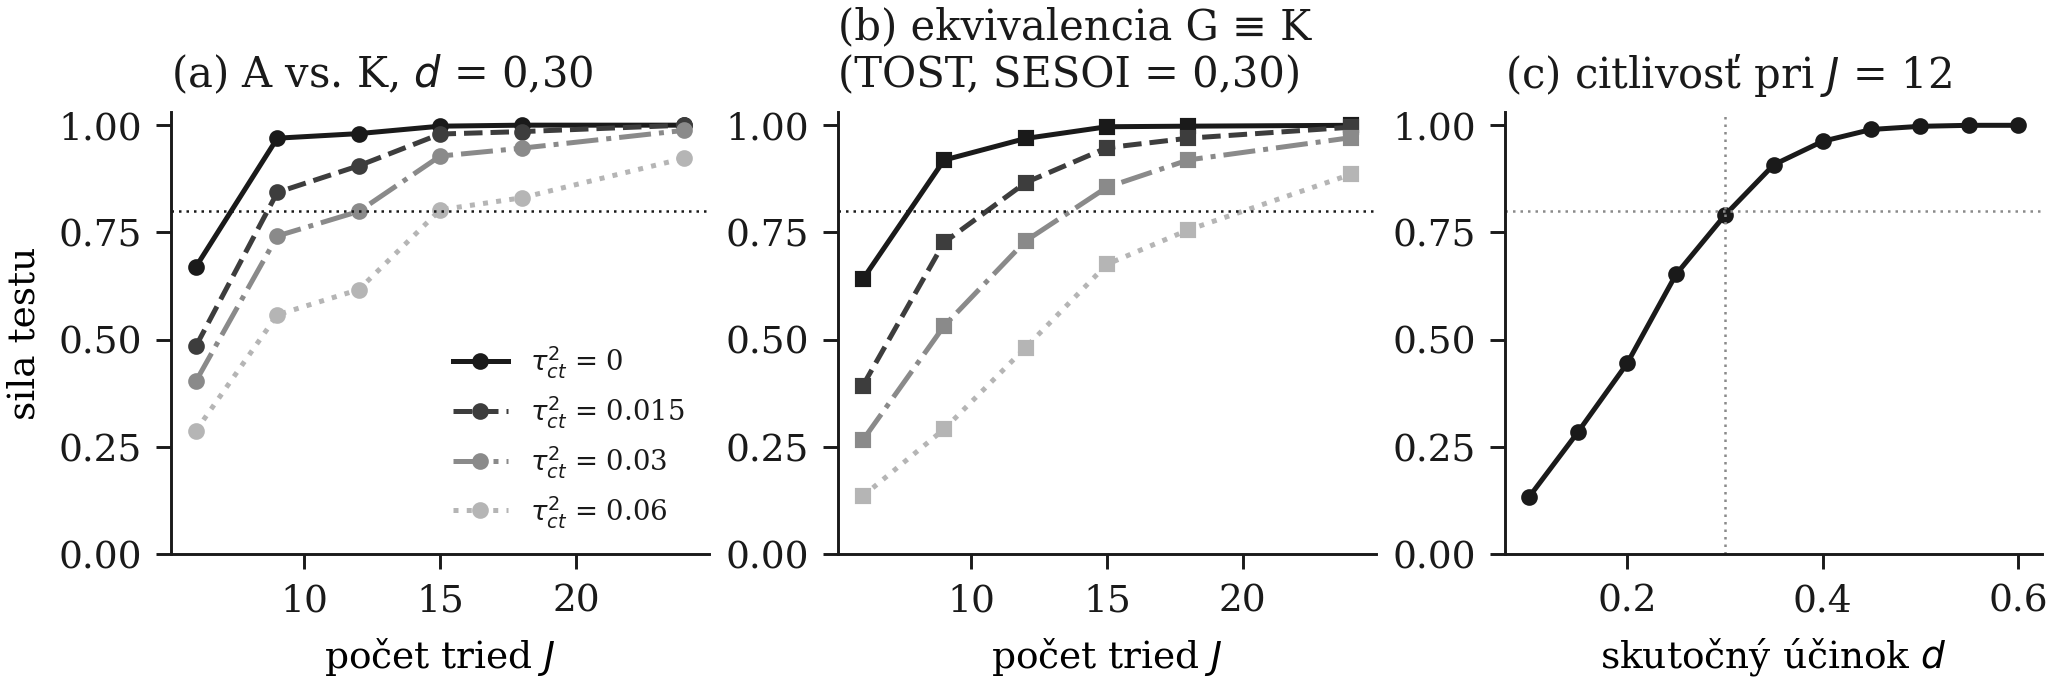
\includegraphics[width=\textwidth]{assets/images/fig_power.png}
    \caption{Sila testu v závislosti od počtu tried $J$ a od heterogenity účinku medzi triedami $\tau^2_{ct}$. (a)~nadradenosť $A$ nad $K$ pri skutočnom účinku $d=0{,}30$; (b)~vyhlásenie ekvivalencie $G\equiv K$ testom TOST; (c)~citlivosť pri $J=12$.}
    \label{fig:sila}
\end{figure}

\paragraph{Kľúčové zistenie.} Rozhodujúcim parametrom nie je počet žiakov, ale \emph{heterogenita účinku medzi triedami} $\tau^2_{ct}$. Pri $\tau^2_{ct}=0$, teda keď je účinok podmienky vo všetkých triedach rovnaký, postačuje 9~tried na silu nad $0{,}95$. Pri realistickej hodnote $\tau^2_{ct}=0{,}03$ klesá sila pri tom istom počte tried na $0{,}74$ a pri $\tau^2_{ct}=0{,}06$ až na $0{,}56$. Dôvodom je, že náhodný účinok podmienky na úrovni triedy sa vo vnútroindividuálnom rozdiele \emph{nevykráti}, a preto sa počet tried stáva viazaným obmedzením~\cite{raudenbush1997cluster}. Z toho vyplýva praktické odporúčanie, ktoré ide proti intuícii: pri danom celkovom počte žiakov je lepšie zapojiť \emph{viac menších tried} než menej veľkých.

\paragraph{Odporúčaná veľkosť vzorky.} Tabuľka~\ref{tab:sila} zhŕňa výsledky pre realistický scenár $\tau^2_{ct}=0{,}03$.

\begin{table}[H]
\centering
\caption{Sila testu pre tri primárne tvrdenia pri $\tau^2_{ct}=0{,}03$, $\rho_{\text{trieda}}=0{,}12$, veľkosti triedy 22 a 12\,\% úbytku}
\label{tab:sila}
\small
\begin{tabular}{@{}lccccccc@{}}
\toprule
$J$ & $N$ zap. & $N$ anal. & $A>K$ & $A>G$ & $G\equiv K$ & rodina & mechanizmus \\
\midrule
6  & \powNsix & \powNasix & \powAKsix & \powAGsix & \powEqsix & \powFamsix & --- \\
9  & \powNnine & \powNanine & \powAKnine & \powAGnine & \powEqnine & \powFamnine & \powMechnine \\
12 & \powNtwelve & \powNatwelve & \powAKtwelve & \powAGtwelve & \powEqtwelve & \powFamtwelve & \powMechtwelve \\
15 & \powNfifteen & \powNafifteen & \powAKfifteen & \powAGfifteen & \powEqfifteen & \powFamfifteen & \powMechfifteen \\
\textbf{18} & \textbf{\powNeighteen} & \textbf{\powNaeighteen} & \textbf{\powAKeighteen} & \textbf{\powAGeighteen} & \textbf{\powEqeighteen} & \textbf{\powFameighteen} & \textbf{\powMecheighteen} \\
24 & \powNtwentyfour & \powNatwentyfour & \powAKtwentyfour & \powAGtwentyfour & \powEqtwentyfour & \powFamtwentyfour & \powMechtwentyfour \\
\bottomrule
\end{tabular}
\vspace{2pt}
\footnotesize „Rodina“ je pravdepodobnosť, že všetky tri konfirmačné testy prejdú Holmovou korekciou súčasne. „Mechanizmus“ je pravdepodobnosť, že odhad dráhy PEQI bude \emph{dosť presný} (95\,\% interval užší než $0{,}20$), nie len významný; jeho odlíšiteľnosť od nuly presahuje $0{,}96$ už pri deviatich triedach (časť~\ref{sec:identifikacia}).
\end{table}

Cieľovou hodnotou je teda \textbf{18~tried}, pri ktorých všetky tri konfirmačné tvrdenia dosahujú silu nad $0{,}90$, celá rodina po Holmovej korekcii $\powFameighteen$ a mechanizmus dosahuje použiteľnú presnosť s pravdepodobnosťou $\powMecheighteen$. Pri 12~triedach je test nadradenosti ešte akceptovateľný ($\powAKtwelve$), ale test ekvivalencie už nie ($\powEqtwelve$) a pravdepodobnosť použiteľne presného mechanizmového odhadu klesá na $\powMechtwelve$. Zber údajov pod 12~tried nemá zmysel začínať.

Za povšimnutie stojí, že posledné dva stĺpce vedú k tomu istému záveru z úplne rôznych smerov. Rodinový stĺpec je viazaný testom ekvivalencie, mechanizmový stĺpec požiadavkou na šírku intervalu. Obidva sa lámu medzi 12 a 15 triedami. Zhoda dvoch nezávislých obmedzení je silnejším argumentom pre veľkosť vzorky než ktorékoľvek z nich samostatne.

\paragraph{Minimálny detegovateľný účinok.} Pri $J=12$ a $\tau^2_{ct}=0{,}03$ je minimálny účinok detegovateľný so silou $0{,}80$ rovný $d=0{,}30$ (obrázok~\ref{fig:sila}~c). Pri $J=18$ klesá na $d\approx0{,}24$.

\paragraph{Operačná charakteristika testu ekvivalencie.} Obrázok~\ref{fig:ekvivalencia} ukazuje, ako sa pravdepodobnosť vyhlásenia ekvivalencie mení so skutočným rozdielom. Pri skutočnom rozdiele $-0{,}20$ klesá pod $0{,}25$, čo je dôležité pre interpretáciu: nevyhlásenie ekvivalencie neznamená dôkaz rozdielu a naopak.

\begin{figure}[H]
    \centering
    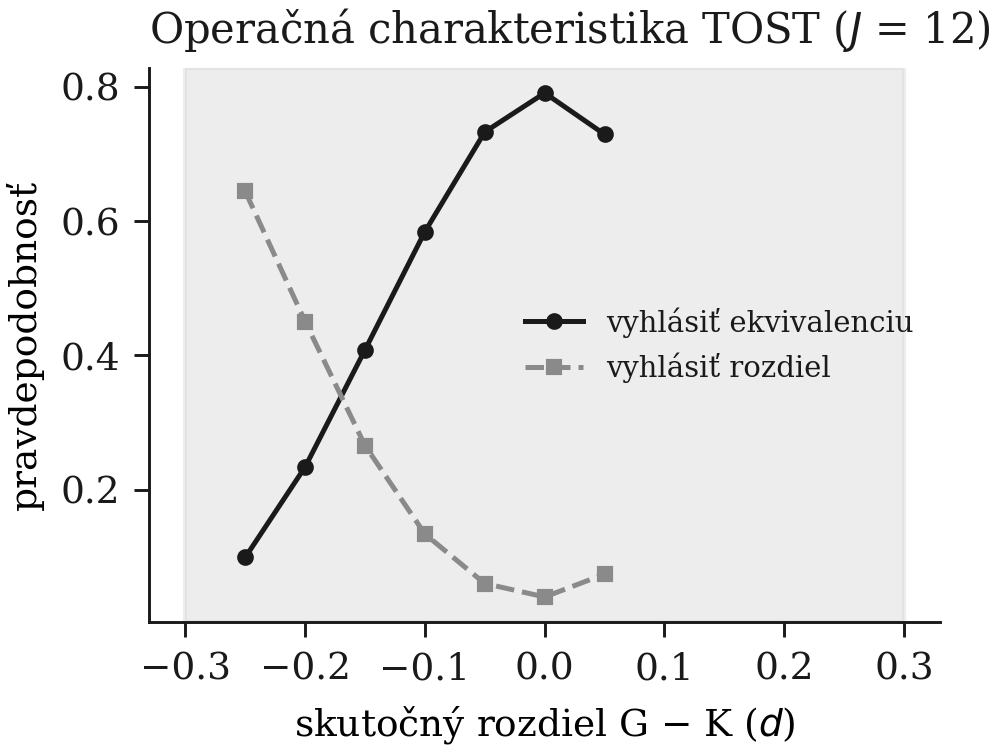
\includegraphics[width=0.62\textwidth]{assets/images/fig_equivalence.png}
    \caption{Operačná charakteristika testu ekvivalencie pri $J=12$. Sivé pásmo vyznačuje pásmo ekvivalencie $\pm0{,}30$.}
    \label{fig:ekvivalencia}
\end{figure}

\section{Validácia metodiky pred zberom údajov}
\label{sec:validacia}

Metodika prechádza pred zberom dát dvoma nezávislými overeniami.

\paragraph{Simulačná validácia analytického plánu.} Celý štatistický plán bol implementovaný a spustený na dátach vygenerovaných z modelu so \emph{známymi} hodnotami parametrov. Zmysel je jednoduchý: čo plán nedokáže odhaliť na simulovaných dátach, neodhalí ani na reálnych. Výsledky tejto validácie sú v kapitole~\ref{chapter:vysledky}. Validácia už priniesla tri konkrétne opravy dizajnu: odhalila spomínanú singularitu v kódovaní prenosu, ukázala, že odložený test s ôsmimi položkami na tému má nedostatočnú spoľahlivosť ($0{,}63$) a viedla k jeho rozšíreniu na dvanásť ($0{,}71$), a kvantifikovala útlm účinkov spôsobený chybou merania.

\subsection{Pilot: čo jedna trieda rozhodne a čo nie}
\label{sec:pilot}

Pilot na jednej triede (približne \pilotN{}~žiakov), ktorá nebude zaradená do hlavnej vzorky, prebehne pred zberom. Pilot bez vopred stanovených rozhodovacích pravidiel je generálna skúška, nie overenie: povie, že hodina prebehla a notebooky fungovali, a hlavná štúdia sa potom ladí podľa vkusu na základe toho, čo pilot náhodou ukázal. Pravidlá preto uvádzame vopred, a spolu s nimi aj to, ktoré otázky vzorka takejto veľkosti \emph{nevie} rozhodnúť.

\begin{table}[H]
\centering
\caption{Rozhodnutia pilotu a ich pravidlá}
\label{tab:pilot}
\scriptsize
\begin{tabularx}{\textwidth}{@{}X X l@{}}
\toprule
\textbf{Otázka} & \textbf{Pravidlo} & \textbf{Rozhodne?} \\
\midrule
Sú obtiažnosti položiek v pásme? & vyradiť položku len ak jej 90\,\% interval leží celý mimo $0{,}30$--$0{,}80$ & slabo \\
Sedí časovanie? & pri prekročení skrátiť blok s najväčšou rezervou, nikdy nie primárny výsledok & \textbf{áno} \\
Funguje záchytná vrstva? & pokrytie pod $0{,}80$ u viac než štvrtiny žiakov $\Rightarrow$ zber sa nezačína & \textbf{áno} \\
Je guard podmienky $A$ tesný? & akýkoľvek únik zastavuje nasadenie & čiastočne \\
Je ICAR spoľahlivý v tejto populácii? & pod $0{,}70$ pridať položky; spúšťa revíziu, nie automatickú zmenu & slabo \\
Sedia lokálne úspešnosti iBoboru s národnými? & systematický rozdiel nad $0{,}3$ logitu rozširuje citlivostné pásmo percentilu & \textbf{áno} \\
Aká je medzitriedna variancia $\tau^2_{ct}$? & preberá sa z literatúry, vykazuje sa citlivosť & \textbf{nie} \\
\bottomrule
\end{tabularx}
\end{table}

\paragraph{Skríning položiek podľa intervalu, nie podľa bodu.} Pôvodné pravidlo znelo: ponechať položky s úspešnosťou medzi $0{,}30$ a $0{,}80$. Pri \pilotN{}~žiakoch je však smerodajná chyba pozorovaného podielu $\pilotSe$, takže toto pravidlo vyradí $\pilotPointGood$ \emph{dobrých} položiek. Každá zbytočne vyradená položka skracuje test, a spoľahlivosť s dĺžkou klesá~--- z $\pilotRelSixteen$ pri šestnástich položkách na $\pilotRelTen$ pri desiatich. Ide teda o trvalú daň na sile hlavnej štúdie, zaplatenú v októbri a splatnú v marci.

Pravidlo preto meníme na intervalové: položka sa vyradí, len ak jej 90\,\% interval leží \emph{celý} mimo pásma. Podiel zbytočne vyradených dobrých položiek klesne na $\pilotIntervalGood$. Cenou je, že podiel odhalených skutočne zlých položiek klesne z $\pilotPointBad$ na $\pilotIntervalBad$~--- a tú cenu prijímame vedome, pretože zlá položka, ktorá pilotom prejde, sa na plnej vzorke odhalí ukazovateľmi zhody s modelom, kým dobrá položka vyradená v pilote je preč natrvalo.

\paragraph{Čo pilot rozhodnúť nemôže.} Plán doteraz uvádzal medzi cieľmi pilotu aj odhad $\tau^2_{ct}$. To je medzitriedna veličina a pilot má \emph{jednu} triedu, takže na jej odhad nemá ani jeden stupeň voľnosti. Hodnota sa preberá z literatúry a plán vykazuje citlivosť naprieč mriežkou hodnôt, čo analýza sily testu už robí.

\paragraph{Čo znamená prejdený guard.} Podmienka nasadenia žiada nulový únik pri \pilotGuardN{} útočných dopytoch. Prejsť ju je nutné, ale nie je to certifikát: nula únikov zo \pilotGuardN{} ohraničuje skutočnú mieru únikov zhora na $\pilotGuardBound$ s 95\,\% spoľahlivosťou, nie na nulu. Pri skutočnej miere únikov 2\,\% prejde sada čistá v $\pilotGuardPass$ prípadov. Na ohraničenie na jedno percento by bolo treba $\pilotGuardNeeded$~dopytov. Preto sa počas zberu vykazuje \emph{pozorovaná} miera porušení guardu zo skutočných relácií: to je číslo, za ktorým stojí sila.

\paragraph{Čo pilot zmeniť nesmie.} Zoznam je krátky a záväzný: SESOI, primárny ukazovateľ, zloženie konfirmačnej rodiny, definície podmienok a voľba analytického modelu. Bez tohto obmedzenia je pilot spôsob, ako štúdiu ladiť dovtedy, kým nesúhlasí s výskumníkom.

\section{Negatívne kontroly: ako by sme zistili, že sa mýlime}
\label{sec:negativne-kontroly}

Dizajn ukáže, že žiaci po adaptívnej hodine skórujú vyššie než po klasickej. Sám osebe neukáže, že sa \emph{naučili} viac. Ten istý kontrast vyrobia aspoň tri mechanizmy, v ktorých sa nikto nenaučil nič navyše:

\begin{description}[leftmargin=0.6cm, nosep]
    \item[\textbf{Očakávanie od účastníka.}] Žiaci vedia, ktorá hodina bola tá „zvláštna“, a tušia, ktorá má vyjsť lepšie. Väčšia snaha na teste, ktorý po nej nasleduje, dvihne \emph{každú} položku toho testu.
    \item[\textbf{Rozdielna zvyšná kapacita.}] Adaptívna hodina je menej vyčerpávajúca, pretože časť záťaže nesie asistent. Žiak prichádza na test s väčšou rezervou~--- a tá sa prejaví na čomkoľvek, aj na učive, ktoré nikdy nevidel.
    \item[\textbf{Okamžitý afekt.}] Hodina, ktorá žiakov bavila, ich zanechá v lepšej nálade, a nálada posúva výkon na nesúvisiacich kognitívnych úlohách.
\end{description}

Všetky tri sú v primárnom kontraste od učenia nerozoznateľné. Všetky tri však predpovedajú niečo, čo učenie nepredpovedá: účinok na látke, ktorú hodina nepokryla. Na tom je postavená falzifikácia.

\subsection{Dve kontroly a to, čo každá sleduje}

\begin{enumerate}[nosep]
    \item \textbf{Placebo položky.} \falPlacebo{} položiek z témy mimo troch skúmaných, zaradených \emph{do toho istého} okamžitého testu, bez upozornenia, že sú iné. Žiadna z troch hodín sa ich nedotkne. Učenie predpovedá nulu; všetky tri alternatívy predpovedajú posun.
    \item \textbf{Nemenná črta.} Skrátený test matíc, zopakovaný na odloženom termíne. Deväťdesiat minút vyučovania nemôže pohnúť fluidným usudzovaním. Účinok tu neznamená zistenie, ale poruchu~--- v prideľovaní, v analýze alebo v administrácii.
\end{enumerate}

Rozdelenie medzi nimi je zámerné a nie je len zdvojením. Placebo položky sa píšu v ten istý deň a v tom istom rozpoložení, takže zachytia okamžitý kanál. Matice sa píšu o tri týždne, takže okamžitý kanál na ne nedosiahne~--- a práve preto zachytia to druhé: chybu v samotnej mašinérii. Zlúčiť ich do jednej kontroly by znamenalo, že úspešne prejdená kontrola hovorí menej, než sa zdá.

\subsection{Prečo je to test ekvivalencie, nie test nulovej hypotézy}

„Pozreli sme sa a nič sme nenašli“ nie je negatívna kontrola; je to malá vzorka. Kontrola je informatívna len vtedy, keď dokáže účinok danej veľkosti \emph{vylúčiť}. Obe kontroly sa preto testujú testom ekvivalencie (TOST) proti hranici $\falBound$, nie testom proti nule.

Hranica je stanovená na rovnakej úrovni ako SESOI primárneho výsledku, a nie prísnejšie. Zvádza zvoliť malé číslo; odolať tomu je poctivejšie, lebo hranica musí byť dosiahnuteľná. Pri 18~triedach je polovičná šírka 90\,\% intervalu na kontrole $\falHalfwidth$, takže hranica $0{,}20$ by ponechala rezervu okolo $0{,}05$ a ekvivalenciu by nevyhlásila zhruba v polovici prípadov, \emph{keď je pravda presne nula}. Kontrola, ktorá v polovici čistých štúdií kričí na poplach, nie je kontrola. Pri hranici $\falBound$ vyhlási ekvivalenciu v $\falPassNull$ prípadov, keď je pravda nula, a falošný poplach nastáva v $\falDetectZero$ prípadov, teda na nominálnej hladine.

Tvrdenie, ktoré kontrola podporuje, je preto presné a treba ho takto aj formulovať: \emph{vylučuje sa kanál mimo učenia dosť veľký na to, aby vysvetlil celý primárny účinok}. Kanál dosť veľký na to, aby vysvetlil jeho časť, sa nevylučuje. Dosiahnuť hranicu $0{,}15$ by si vyžiadalo približne štvornásobok tried, čo je výmena, ktorú táto štúdia urobiť nemôže.

\begin{table}[H]
\centering
\caption{Sila negatívnej kontroly proti úniku mimo učenia rôznej veľkosti ($J=18$, \falPlacebo{} placebo položiek)}
\label{tab:negkontrola}
\small
\begin{tabular}{@{}lccccc@{}}
\toprule
veľkosť úniku & 0,00 & 0,10 & 0,20 & 0,30 & 0,45 \\
\midrule
kontrola sa ozve & \falDetectZero & \falDetectTen & \falDetectTwenty & \falDetectThirty & \falDetectFortyFive \\
vyhlási sa ekvivalencia & \falEquivZero & \falEquivTen & \falEquivTwenty & \falEquivThirty & \falEquivFortyFive \\
\bottomrule
\end{tabular}
\end{table}

Tabuľka~\ref{tab:negkontrola} sa číta po stĺpcoch a obsahuje dve rôzne otázky. Prvý riadok je pravdepodobnosť, že sa ozve poplach; druhý je pravdepodobnosť, že kontrola vyhlási čisto. Dobrá kontrola má prvý riadok rastúci a druhý klesajúci~--- keby pri veľkom úniku zostal druhý riadok vysoký, prejdená kontrola by neznamenala nič. Pri úniku veľkosti primárneho účinku ($0{,}30$) sa kontrola ozve v $\falDetectThirty$ prípadov a ekvivalenciu vyhlási len v $\falEquivThirty$.

Kontrola nemennou črtou prejde v $\falTraitPass$ prípadov aj vtedy, keď je okamžitý kanál naplno otvorený, a falošne sa ozve v $\falTraitAlarm$~--- čo je presne to, čo má robiť kontrola citlivá na poruchu mašinérie a necitlivá na motiváciu v deň testu.

\paragraph{Koľko položiek sa oplatí vytlačiť.} Výnosy klesajú rýchlo a dôvod je poučný. Kontrast je vnútroindividuálny, takže zvyškom je zložka žiak\,$\times$\,príležitosť, a vzorkovanie položiek je len jednou jej časťou; viac položiek zmenšuje tú jednu časť. Pri \falShortItems{} položkách je polovičná šírka $\falHalfShort$, pri \falPlacebo{} $\falHalfwidth$ a pri \falLongItems{} už len $\falHalfLong$. Takmer štyri pätiny dosiahnuteľnej presnosti sú teda na mieste do deviatej položky; zvyšok stojí čas hodiny, ktorý potrebuje primárny výsledok.

\subsection{Vopred stanovené rozhodovacie pravidlo}

Ak ktorákoľvek z oboch kontrol ekvivalenciu \emph{nevyhlási}, primárny kontrast sa vykazuje spolu s vysvetlením mimo učenia uvedeným vedľa neho a mechanizmové tvrdenie sa sťahuje. Dôvod je vecný: výhoda na neprebratej látke získaná v ten istý deň nie je učenie, a ak je prítomná, nemožno tvrdiť, že primárny účinok učením je. Pravidlo je stanovené teraz práve preto, aby sa o ňom nerozhodovalo podľa toho, ako výsledok vyjde.


\section{Ohrozenia validity a ich ošetrenie}
\label{sec:validita}

Tabuľka~\ref{tab:ohrozenia} sumarizuje ohrozenia validity v členení podľa Shadisha, Cooka a Campbella~\cite{shadish2002experimental} spolu s konkrétnym opatrením a spôsobom, akým jeho účinnosť overujeme. Zoznam je zámerne úplný vrátane ohrození, ktoré ošetriť nevieme.

\begin{table}[H]
\centering
\caption{Ohrozenia validity, opatrenia a overenie účinnosti}
\label{tab:ohrozenia}
\scriptsize
\begin{tabularx}{\textwidth}{@{}l X X@{}}
\toprule
\textbf{Ohrozenie} & \textbf{Opatrenie} & \textbf{Overenie} \\
\midrule
Prenos medzi periódami & 6 sekvencií, týždenný odstup, obsahovo nezávislé témy & parameter prenosu v modeli; model len na 1.~perióde \\
Zámena témy a podmienky & latinský štvorec & interakcia podmienka $\times$ perióda \\
Efekt novosti nástroja & 3 periódy; položka o vnímanej novosti & novosť ako kovariát; trend cez periódy \\
Efekt experimentátora & skriptovaný výklad, ten istý učiteľ, notebooky vo všetkých podmienkach & protokol vernosti \\
Kontaminácia podmienky $K$ & zoznam povolených adries, pozorovateľ, samostatný dotazník & analýza podľa priradenia verzus podľa priebehu \\
Testovací efekt & konštantný naprieč podmienkami & uvedený pri interpretácii absolútnych hodnôt \\
Neekvivalentné formy testov & spoločné kotviace položky, Raschovo prepojenie & analýza funkčnej odlišnosti položiek \\
Stropový a podlahový efekt & pilot s cieľovou obtiažnosťou 0,30--0,80 & rozdelenie úspešnosti položiek \\
Útlm účinku chybou merania & dostatočný počet položiek, Raschova škála & vykazovanie s korekciou aj bez nej \\
Diferenciálny úbytok & sledovanie podľa podmienky & porovnanie vstupných charakteristík; imputácia \\
Heterogenita účinku medzi triedami & modelovaná, nie predpokladaná & náhodný sklon; zahrnutie do výpočtu sily \\
Zámerný výber škôl & stratifikácia podľa typu a lokality & otvorene priznané obmedzenie \\
Neviditeľné použitie na vlastnom zariadení & meranie miery pokrytia & citlivostná analýza bez nekonzistentných prípadov \\
Nepozorované zmätenie mediátora a výsledku & mechanizmus nie je v konfirmačnej rodine; triangulácia troch odhadov & analýza citlivosti $\rho^\ast$ s vopred stanoveným prahom \\
Porušenie podmienky vylúčenia pri inštrumente & podmienky $G$ a $A$ zdieľajú model, úlohy, rozhranie aj učiteľa & vymenované zvyšné kanály; odhad vykázaný ako horná hranica \\
Výpadok závislý od schopnosti & vstupné vedomosti v modeli & test MCAR, viacnásobná imputácia, nepriaznivý scenár \\
Neekvivalentné kalibrácie foriem & súbežná kalibrácia cez kotviace položky & overenie obnovenia veľkosti zabudnutia \\
Jediná doména učiva & --- & priznané obmedzenie; návrh nadväzujúceho výskumu \\
\bottomrule
\end{tabularx}
\end{table}

\section{Etické a právne aspekty}
\label{sec:etika}

Výskum sa týka neplnoletých osôb a zahŕňa zachytávanie sieťovej prevádzky. Obidve okolnosti zvyšujú nároky nad rámec bežného školského výskumu. Úplná dokumentácia vrátane vzorov súhlasov a analýzy vplyvu na ochranu údajov je v prílohe~\ref{chapter:etika}.

\paragraph{Súhlas.} Vyžaduje sa písomný súhlas zákonného zástupcu a samostatný súhlas žiaka v jazyku primeranom veku. Odvolanie súhlasu je možné kedykoľvek bez udania dôvodu a bez následkov; žiak sa naďalej zúčastňuje vyučovania, len sa jeho dáta nespracúvajú. Účasť nemá žiadny vplyv na známku.

\paragraph{Právny základ a minimalizácia.} Právnym základom je súhlas podľa článku 6 ods. 1 písm. a) v spojení s článkom 8 nariadenia GDPR~\cite{gdpr2016} a zákona č.~18/2018 Z.~z.~\cite{zakon18_2018}. Zachytávajú sa výhradne telá požiadaviek smerujúcich na adresy zo zoznamu povolených; ostatná prevádzka sa nespracúva a neukladá. Odpovede modelu sa neukladajú doslovne, ale vo forme odtlačku a dĺžky, ktoré postačujú na výpočet VTR bez uchovávania obsahu.

\paragraph{Pseudonymizácia.} Identifikátor žiaka sa nahrádza hašom so soľou, ktorú uchováva škola a výskumník k nej nemá prístup. Text promptov prechádza pred uložením odstraňovaním osobných údajov (vzory pre mená, adresy, rodné čísla, kontakty) a jeho úspešnosť sa vykazuje na ručne anotovanej vzorke.

\paragraph{Analýza vplyvu na ochranu údajov.} Keďže ide o systematické monitorovanie a o dáta detí, vykonáva sa posúdenie vplyvu podľa článku 35 GDPR. Certifikačná autorita sa inštaluje výlučne na školské zariadenia zapojené do štúdie a po jej skončení sa preukázateľne odstraňuje; žiaci vidia na začiatku každej relácie viditeľné upozornenie, že prevádzka je pre účely výskumu zaznamenávaná.

\paragraph{Akt o umelej inteligencii.} Adaptívny tutor hodnotí učebné výsledky, čo je činnosť uvedená v prílohe~III nariadenia~\cite{euaiact2024}. Systém je nasadený výlučne na výskumné účely a nemá vplyv na hodnotenie žiaka, čím sa naň vzťahuje výnimka pre výskumnú a vývojovú činnosť. Práca napriek tomu dokumentuje systém tak, ako keby sa naň požiadavky vzťahovali~--- opis údajov, opis obmedzení, ľudský dohľad~--- pretože v prípade prechodu do školskej praxe by to bolo nevyhnutné.

\paragraph{Schválenia.} Pred začatím zberu sa vyžaduje stanovisko etickej komisie STU, súhlas riaditeľa každej zapojenej školy a informovanie rodičovskej rady. Predregistrácia dizajnu a analytického plánu sa vykonáva vo verejnom registri pred prvým meraním~\cite{nosek2018preregistration}.
